\title{Implementing a MIPS processor using SME}
\author{Carl-Johannes Johnsen (grc421)}
%% Skabelon til LiCS-afleveringer

%%%%%%%%%%%%%%%%%%%%%%%%%%%%%%%%%%%%%%%%%%%%%%%%%%%%%%%%%%%%%%%
%% Begynd preamble
%%%%%%%%%%%%%%%%%%%%%%%%%%%%%%%%%%%%%%%%%%%%%%%%%%%%%%%%%%%%%%%
\documentclass[a4paper]{article}

%% Til at tegne træer!
\usepackage{tikz}
\usetikzlibrary{positioning,arrows,calc}
\tikzset{
    on grid,
    node distance=3cm,
    auto,
    block/.style = {
        draw,
        shape=rectangle,
        minimum height=3em,
        minimum width=3em,
        line width=1pt
    },
    control/.style = {
        draw,
        shape=circle,
        minimum height=7em,
        minimum width=3em,
        line width=1pt
    },
    mux/.style = {
        draw,
        shape=rectangle,
        minimum height=1.5em,
        minimum width=1em,
        line width=1pt
    },
    empty/.style = {
        shape=rectangle,
        minimum height=3em,
        minimum width=3em
    },
    >=latex',
}

%% Til at kunne have billeder
\usepackage{graphicx}
%% Til at kunne have source code
\usepackage{listings}
\lstset{
  breaklines=true,
  keepspaces=true,
  frame=ltrb,
  framesep=1pt,
  commentstyle=\color{Brown},
  basicstyle=\ttfamily\footnotesize,
  numbers=left,
  title=\lstname,
  columns=fullflexible,
  extendedchars=\true,
  inputencoding=ansinew,
}

%% Font and input encoding
%% Tillad æøå
\usepackage[T1]{fontenc}
\usepackage[utf8]{inputenc}
%% Babel (language)
\usepackage[UKenglish]{babel} % If you write in English
\usepackage[UKenglish]{isodate}
%\usepackage{parskip}
\usepackage{booktabs}
%\usepackage[danish]{babel} % Hvis du skriver på dansk

%% Til links
\usepackage{hyperref}
\usepackage{subfig}

%% AMS-Math packages
\usepackage{amsmath}
\usepackage{amssymb}
\usepackage{amsthm}
\newtheorem{theorem}{Theorem}
%% Extra symbols that we almost always need
\usepackage{stmaryrd}
\usepackage{color}
\usepackage{url}
\usepackage{semantic}
\usepackage{fancyref}
\usepackage{enumitem}

%%%%%%%%%%%%%%%%%%%%%%%%%%%%%%
%% Skift sidenumrene ud med X/total (lettere at rette :-)
\usepackage{lastpage}
\makeatletter
\renewcommand{\@oddfoot}{\hfil \thepage{}/\pageref{LastPage} \hfil}
\renewcommand{\@evenfoot}{\hfil \thepage{}/\pageref{LastPage} \hfil}
\makeatother
%%%%%%%%%%%%%%%%%%%%%%%%%%%%%%

% Til at få tabeller mindre?
\usepackage{adjustbox}

% Til klasse diagrammer
%\usepackage{pgf-umlcd}
%\renewcommand{\umldrawcolor}{black}
%\renewcommand{\umlfillcolor}{white}
%\let\classoperation\operation

% forkortelse af texttt!
\renewcommand{\bf}{\textbf}
\renewcommand{\tt}{\texttt}
\renewcommand{\sf}{\textsf}
\renewcommand{\it}{\textit}
\newcommand{\E}{\mathbb{E}}

% Forkortelser som bruger tt!
\newcommand{\tif}{\tt{ if }}
\newcommand{\tthen}{\tt{ then }}
\newcommand{\telse}{\tt{ else }}
\newcommand{\tfalse}{\tt{ false }}

%%%%%%%%%%%%%%%%%%%%%%%%%%%%%%%%%%%%%%%%%%%%%%%%%%%%%%%%%%%%%%%
%% Slut preamble -- herunder følger selve dokumentet!
%%%%%%%%%%%%%%%%%%%%%%%%%%%%%%%%%%%%%%%%%%%%%%%%%%%%%%%%%%%%%%%
\sloppy
\begin{document}
\maketitle

% TODO !!!
% Appendix
% Fix github

\begin{abstract}
    The Synchronous Message Exchange (SME) model, is a programming model, which
    closely resembles the CSP model and which is suitable for describing
    hardware. This thesis aims to combine the theory taught in a machine
    architecture class with the SME model, by implementing a MIPS processor
    using SME. I show how to construct the components of a MIPS processor as
    SME processes, and how to connect them by using SME busses. Furthermore, I
    show how to extend the processor, by introducing additional instructions
    and by pipelining the processor. Finally, I succesfully implement the
    Single Cycle and Pipelined MIPS processors onto an FPGA. \\

    \noindent
    Thesis supervisors: Brian Vinter and Kenneth Skovhede.
\end{abstract}

\newpage
\section*{Acknowledgements}
I would like to acknowledge my thesis supervisors Brian Vinter and Kenneth
Skovhede for guiding me through writing my thesis and through writing the
corresponding paper~\cite{ref:cpa-paper}. I would also like to thank the
employees in the eScience group at the Niels Bohr Institute, for taking their
time to listen to my project and give me feedback on my progress. Finally,
thanks to Daniel Lundberg Pedersen and Jeanette Johnsen for proof reading.

\newpage
\tableofcontents
\newpage

% \section*{Spørgsmål}
% \begin{enumerate}
%   \item Istedet for at have alle baggrunds teorien løbende, så tænkte jeg om der skulle
%     være et afsnit, som gennemgår al teorien?

%   \item Skal jeg have mere CSP teori med? I så fald medfører det vel også noget SME teori. - tjek intro

%   \item Skal jeg, og i så fald hvordan, referere min egen artikel? Eller skal jeg skynde mig at skrive den om, så de ikke er lig hinanden? - related work

%   \item Er det sidste afsnit om "Synthesizing" lidt for specifik?

%   \item Er de andre afsnit for uspecifikke?

%   \item Skal related work være et afsnit i introduction, eller skal det bare flettes ind i introduction? eller skal det et helt andet sted hen? Eget afsnit
% \end{enumerate}

% SME mangler!: Dobbelt tjek at de er med i rapporten, da det er nogle af de fund jeg har lavet!
% \begin{itemize}
%   \item AXI interface

%   \item Standard typer til top-level busser (pga block design ikke kan lide
%     custom typer)

%   \item Signal splitting

%   \item Caste et tal til en enum.
% \begin{lstlisting}
% control.opcode = (Opcode) ((instruction >> 26) & 0x3F);
% \end{lstlisting}
% skal lave VHDL:
% \begin{lstlisting}
% ControlIn_opcode <= SingleCycleMIPS_Opcodes'VAL(TO_INTEGER(UNSIGNED(instruction(31 downto 26))));
% \end{lstlisting}

%   \item Processer inde i klasser. Transpileren kan ikke lide navnene!
% \begin{lstlisting}
% public class ID
% {
%   public class Splitter : SimpleProcess
%   {
%   ...
% \end{lstlisting}

%   \item Lidt resikabelt at være ude i det, men muligheden for at kunne lave
%     noget, som kun kørte når clocken er høj, lav, rising edge eller falling edge?
%     Kunne f.eks. være noget ala OnHigh(). Lidt ligesom at det er lidt misvisende
%     at ikke clockede processer kalder det OnTick(), selv om der ikke er noget tick.

%   \item Der kan opstå fejl i Vivado, hvis man har et signal, som både skal gå
%     iblandt flere processer, men samtidig skal gå ud som top-level. Dette kan
%     fikses, ved at have et \texttt{signal} i den VHDL fil, som sørger for at
%     forbinde alt det indre, og at processerne så er forbundet til det signal,
%     istedet for andre forbindelser.
% \end{itemize}

\section{Introduction}
\subsection{Software requirements for using SME}
SME is a library for \tt{C\#}. Therefor we need to setup a development
environment for \tt{C\#}. We will be using \tt{mono} URL % TODO

Now that we have \tt{mono} installed, we need to download and run \tt{SME}. We
start by cloning the project from github: URL!. % TODO
Then, we add the project in
\tt{monodevelop}. Before building the project, we need to generate a few files
(\tt{SME.Render.VHDL/Entity.tt} and \tt{SME.Render.VHDL/TopLevel.tt},
which is done by right clicking the file, and choosing 'Tools > Process T4
Template'. Finally, we can open one of the example programs, and press f5 to
build and run.

%install monodevelop
%clone from github
%run process T4 template on SME.Render.VHDL/Entity.tt and
%SME.Render.VHDL/TopLevel.tt
%Open example project, and press f5 to build and run

\subsection{Logic gates}
To start with, I am going to implement the 4 basic logic gates: \tt{AND},
\tt{OR}, \tt{NOT} and \tt{XOR}, as these are the basic building blocks of a
processor.

I start by describing the busses. I have one input bus, which has two fields:
\tt{Bit1} and \tt{Bit2}, and an output bus, which has four fields, one for each
gate. Note that these interfaces has to be public
%%\lstinputlisting{Buses.cs}

Then I define the processes for each of the logic gates. They are very simple,
as they just take the two inputs, applies their logic operation, and puts the
output on the designated lane on the output bus.
%\lstinputlisting{Gates.cs}

Finally, I wrote a test process, which feeds input to the gate processes,
stores the output from the gate processes, and finally verifies the collected
results, which is:
\begin{tabular}{cc|cccc}
    \tt{Bit1} & \tt{Bit2} & \tt{AND} & \tt{OR} & \tt{NOT} & \tt{XOR} \\
    \hline
    false     & false     & false    & false   & true     & false \\
    false     & true      & false    & true    & true     & true  \\
    true      & false     & false    & true    & false    & true  \\
    true      & true      & true     & true    & false    & false \\
    \hline
\end{tabular}
%\lstinputlisting{GateTester.cs}

\subsection{Decoder}
A decoder takes an $n$-bit input, and has $2^n$ outputs. Exactly one of the
outputs are \tt{1} on any given input. If the value of the input is \tt{0}, then
bit0 of the output is set to \tt{1}, and the rest is set to \tt{0}. If the
value of the input is 124, then bit124 is set to \tt{1}, and the rest is set to
\tt{0}.

I have implemented a 2-bit encoder, by having 2 \tt{NOT} gates, and 4 \tt{AND}
gates:
% TODO figurer!!!

\subsection{Scalable Decoder}
The previous decoder was a hardcoded decoder, i.e. that I had manually defined
all of the busses and the processes. Since SME requires that everything is
known at compile time, we have to define everything statically. This results in
an exponential amount of work when making a larger decoder, where the work is
primarely defining the buses, each has to have an unique name, and defining the
processes, as each has to read from a different bus, or in another case, read
from a different wire on the bus.

To solve this, I have used T4 Templates to generate the source code files for
me, since the network is just a bunch of busses, \tt{NOT} gates and \tt{AND}
gates.

\subsection{Half adder}
A half adder is a circuit, which takes 2 inputs, each one bit, and adds them
together, outputting a sum bit and a carry bit.

\subsection{Full adder}
A full adder is a circuit, which takes 3 inputs, each one bit, and adds them
together, outputting a sum bit, and a carry bit. The difference between a half
adder and a full adder is the extra input, which is designated to be the carry
from the previous full adder in a chain of adders.

\subsection{32 bit adder}
Now that I have made scalable \tt{SME} networks, an half adder and a full
adder, I can make a 32 bit adder. The 32 bit adder starts with an half adder
connected to the first bit of the first input number and to the first bit of
the second input number. The output of the half adder is the first bit of the
output. The remainder of the adder consists of 31 full adders, where we say
that the $i$th full adder is connected to the $i$th bit of both of the input
numbers, to the carry from the $i-1$th adder, and outputs the $i$th bit of the
result, and the $i$th carry. The last carry is the flag indicating whether or
not the addition produced an overflow.

I have made the implementation using Templates, and as such, we can also use
this to produce an $n$-bit adder, just by changing the \tt{BitWidth} variable
of each of the template files.


% Remember! newpage on new chapters
%\newpage
%\section{Getting started with SME}
%\subsection{Installing SME}
\subsection{Writing first SME program}
\subsection{C\# and bit hacking}
\subsection{Translating first SME program into VHDL}
\subsection{Running and verifying VHDL}


%\newpage
\section{Basic logic circuits}
\label{sec:logic-circuits}
In this section, I will be looking at some basic combinatorial circuits. I
start by looking at some logic gates, which implement some boolean functions.
% TODO: omskriv vil jeg mene!
All of the considered values in the system are binary, e.g. the logic gates
works on \texttt{1}s and \texttt{0}s.

\subsection{Basic logic gates}
Start by defining the basic logic gates, which are common for most circuits. A
logic gate is a circuit abstraction, which has inputs and outputs. Its output
values are based upon the input values.

\begin{description}
    \item[\texttt{AND}] - outputs \texttt{1} iff. all of its inputs are
        \texttt{1}, otherwise it outputs \texttt{0}.

    \item[\texttt{OR}] - outputs \texttt{1} if one or more of its inputs are
        \texttt{1}, otherwise it outputs \texttt{0}.

    \item[\texttt{NOT}] -outputs the inverse of its input, i.e. \texttt{1}
        becomes \texttt{0} and \texttt{0} becomes \texttt{1}.

    \item[\texttt{XOR}] - outputs \texttt{1} iff exactly one of its inputs are
        \texttt{1}, otherwise it outputs \texttt{0}
\end{description}
The full truth table for all of the four logic gates can be seen in Table
\ref{tab:truth-table}

\begin{table}
    \centering
    \begin{tabular}{cc|cccc}
        \toprule
        \texttt{Bit1} & \texttt{Bit2} & \texttt{AND} & \texttt{OR} &
        \texttt{NOT} & \texttt{XOR} \\
        \midrule
        false     & false     & false    & false   & true     & false \\
        false     & true      & false    & true    & true     & true  \\
        true      & false     & false    & true    & false    & true  \\
        true      & true      & true     & true    & false    & false \\
        \bottomrule
    \end{tabular}
    \caption{The truth table for the four basic logic gates. Note: \texttt{NOT}
    is only considering \texttt{Bit1}.}
    \label{tab:truth-table}
\end{table}

\subsubsection{Implementation}
Implementing each of these four logic gates is quite simple: There is an input
bus with two 1-bit values, a process for each of the gates, and an output bus
with a 1-bit value for each of the logic gates. % (See Figure
%\ref{fig:logic-gate}).
%
%\begin{figure}
%    \centering
%    \begin{tikzpicture}
%        \coordinate(input);
%        \node[block, right of=input] (A) {Logic gate};
%        \path[->] (input) edge node [midway, above] {input} (A);
%        \node[right of=A] (output) {};
%        \path[->] (A) edge node [midway, above] {output} (output);
%    \end{tikzpicture}
%    \caption{The structure of a Logic gate process}
%    \label{fig:logic-gate}
%\end{figure}

\subsubsection{Testing}
To test the four processes, I have made a process, which sets the bits to all
of the values in the truth table, and checks whether or not each process
outputs the expected value from the truth table. How the processes are
connected can be seen in Figure \ref{fig:logic-test}.

\begin{figure}
    \centering
    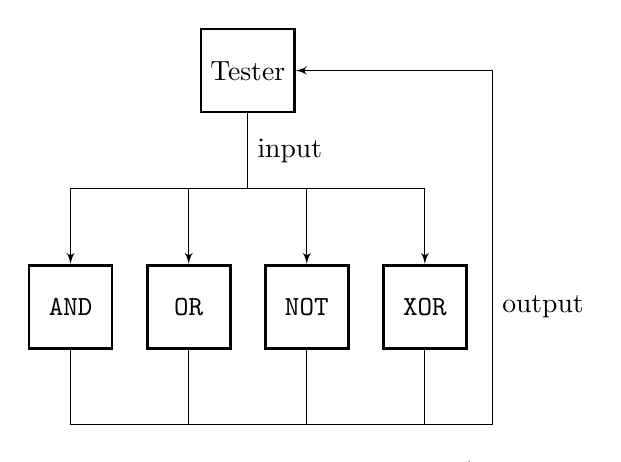
\begin{tikzpicture}[node distance=1.5cm]
        \node[block] (and) {\texttt{AND}};
        \node[block, right of=and] (or) {\texttt{OR}};
        \node[block, right of=or] (not) {\texttt{NOT}};
        \node[block, right of=not] (xor) {\texttt{XOR}};
        \node[above of=and] (input) at ($(or)!0.5!(not)$) {};
        \node[block, above of=input] (tester) {Tester};

        \path[-] (tester) edge node[midway, right] {input} (input.center);
        \path[draw, ->] (input.center) -| (and.north);
        \path[draw, ->] (input.center) -| (or.north);
        \path[draw, ->] (input.center) -| (not.north);
        \path[draw, ->] (input.center) -| (xor.north);

        \node[below of=and] (output) at ($(or)!0.5!(not)$) {};
        \node[right of=xor] (a) {output};

        \path[draw, -] (and.south) |- (output.center);
        \path[draw, -] (or.south) |- (output.center);
        \path[draw, -] (not.south) |- (output.center);
        \path[draw, -] (xor.south) |- (output.center);

        \path[draw, -] (output.center) -| (a.west);
        \path[draw, ->] (a.west) |- (tester.east);
    \end{tikzpicture}
    \caption{The structure of the test of the logic gates}
    \label{fig:logic-test}
\end{figure}

\subsection{Decoder}
% TODO 0-indexed!
The first combinatorial circuit I make is the decoder. An decoder takes an
$n$-bit input, and produces an $2^n$-bit output, where the bit corresponding to
the input numbers value is set to \texttt{1}. E.g. if the input value is the
binary representation of the number 5, then the 5th output bit will be
\texttt{1}, and the rest will be \texttt{0}.

A decoder can be made from a set of \texttt{NOT} and \texttt{AND} gates. We
need to have $n$ \texttt{NOT} gates, and $2^n$ \texttt{AND} gates. For each
input, we split it into two, and send the copy to a \texttt{NOT} gate. Then for
each output, we attach an \texttt{AND} gate, and give it inputs corresponding
to the binary representation of the number %TODO mangler ord.
E.g. if we get the number 5, the binary representation is 101, i.e. the 5th
\texttt{AND} gate gets input from Bit0, \texttt{NOT} Bit1 and Bit2. An example
of a 2-bit decoder can be seen in Figure \ref{fig:2-bit-decoder}.

\begin{figure}
    \centering
    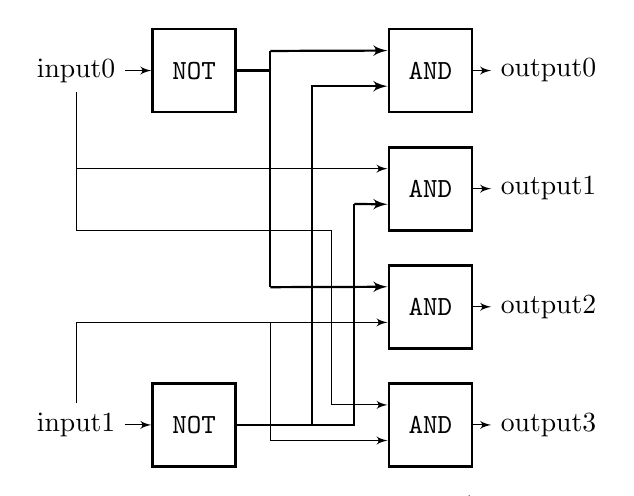
\begin{tikzpicture}[node distance=1.5cm]
        \node[block] (and0) {\texttt{AND}};
        \node[block, below of=and0] (and1) {\texttt{AND}};
        \node[block, below of=and1] (and2) {\texttt{AND}};
        \node[block, below of=and2] (and3) {\texttt{AND}};

        \node[right of=and0] (output0) {output0};
        \node[right of=and1] (output1) {output1};
        \node[right of=and2] (output2) {output2};
        \node[right of=and3] (output3) {output3};

        \path[draw, ->] (and0) -- (output0);
        \path[draw, ->] (and1) -- (output1);
        \path[draw, ->] (and2) -- (output2);
        \path[draw, ->] (and3) -- (output3);

        \node[empty, left of=and0] (andinp0) {};
        \node[empty, left of=and1] (andinp1) {};
        \node[empty, left of=and2] (andinp2) {};
        \node[empty, left of=and3] (andinp3) {};

        \node[block, left of=andinp0] (not0) {\texttt{NOT}};
        \node[block, left of=andinp3] (not1) {\texttt{NOT}};

        \node[left of=not0] (input0) {input0};
        \node[left of=not1] (input1) {input1};

        \path[draw, ->] (input0) -- (not0);
        \path[draw, ->] (input1) -- (not1);

        \path[draw, thick, -] (not0) -| (andinp0.155);
        \path[draw, thick, ->] (andinp0.155) -- (and0.155);
        \path[draw, thick, -] (not1.east) -| (andinp0.south);
        \path[draw, thick, ->] (andinp0.south) |- (and0.200);

        \path[draw, ->] (input0) |- (and1.155);
        \path[draw, thick, -] (not1.east) -| (andinp1.340);
        \path[draw, thick, ->] (andinp1.340) -- (and1.200);

        \path[draw, thick, -] (not0.east) -| (andinp2.155);
        \path[draw, thick, ->] (andinp2.155) -- (and2.155);
        \path[draw, ->] (input1.north) |- (and2.200);

        \path[draw, -] (input0) |- (andinp1.295);
        \path[draw, ->] (andinp1.295) |- (and3.155);
        \path[draw, -] (input1) |- (andinp2.200);
        \path[draw, ->] (andinp2.200) |- (and3.200);

    \end{tikzpicture}
    \caption{An 2-bit decoder made by \texttt{AND} and \texttt{NOT} gates.}
    \label{fig:2-bit-decoder}
\end{figure}

%\subsubsection{$n$-bit decoder}
\subsubsection{Testing}
I have written both a 2-bit decoder, and an $n$-bit decoder. They are tested in
the same fashion as the logic gates, i.e. a tester process is connected to the
input and output bus. The test inputs every combination of numbers, i.e. $2^n$,
and checks after each input, that the correct output is set to \texttt{1} and
\texttt{0} respectively.

\subsection{Adder}
As with the decoder, an adder can be constructed by a combination of
\texttt{AND}, \texttt{OR} and \texttt{XOR} gates. An $n$-bit adder is a chain
of two major components: an half adder and a full adder.

The half adder is the initial component in the chain. It takes two binary
inputs, and outputs the sum and the carry of the addition (See Figure
\ref{fig:half-adder}.

The rest of the $n$-bit adder consists of a chain of full adders, that take
three inputs, A, B, and the carry from the previous link in the chain, and
outputs the sum and the carry of the addition (See Figure
\ref{fig:full-adder}).

The combination of the components can be seen in Figure \ref{fig:n-bit-adder}.


\begin{figure}
    \centering
    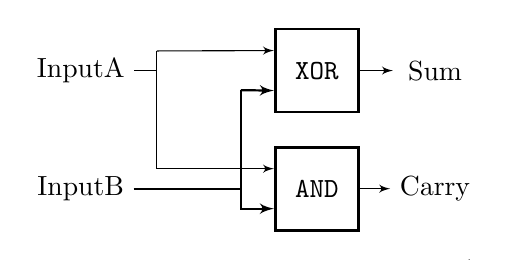
\begin{tikzpicture}[node distance=1.5cm]
        \node[block] (xor) {\texttt{XOR}};
        \node[block, below of=xor] (and) {\texttt{AND}};

        \node[empty, left of=xor] (xorin) {};
        \node[empty, left of=and] (andin) {};

        \node[left of=xorin] (inputa) {InputA};
        \node[left of=andin] (inputb) {InputB};

        \node[empty, right of=xor] (sum) {Sum};
        \node[empty, right of=and] (carry) {Carry};

        \path[draw, -] (inputa) -| (xorin.155);
        \path[draw, ->] (xorin.155) -- (xor.155);
        \path[draw, ->] (xorin.west) |- (and.155);

        \path[draw, thick, -] (inputb.east) -| (xorin.335);
        \path[draw, thick, ->] (xorin.335) -- (xor.205);
        \path[draw, thick, ->] (andin.east) |- (and.205);

        \path[draw, ->] (xor) -- (sum);
        \path[draw, ->] (and) -- (carry);
    \end{tikzpicture}
    \caption{An half adder composed of \texttt{XOR} and \texttt{AND} gates}
    \label{fig:half-adder}
\end{figure}

\begin{figure}
    \centering
    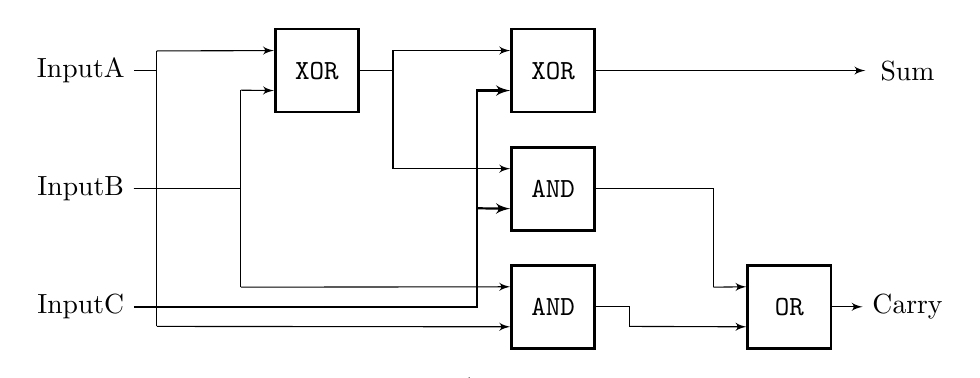
\begin{tikzpicture}[node distance=1.5cm]
        \node[block] (or) {\texttt{OR}};
        \node[empty, left of=or] (orin) {};
        \node[block, left of=orin] (and1) {\texttt{AND}};
        \node[block, above of=and1] (and0) {\texttt{AND}};
        \node[empty, left of=and0] (and0in) {};
        \node[block, above of=and0] (xor1) {\texttt{XOR}};
        \node[empty, left of=xor1] (xor1in) {};
        \node[block, left of=xor1in] (xor0) {\texttt{XOR}};
        \node[empty, left of=xor0] (xor0in) {};
        \node[empty, left of=xor0in] (inputa) {InputA};
        \node[empty, below of=inputa] (inputb) {InputB};
        \node[empty, below of=inputb] (inputc) {InputC};
        \node[empty, right of=inputc] (inputcout) {};
        \node[empty, right of=xor1] (sum) {};
        \node[empty, right of=sum] (summ) {};
        \node[empty, right of=summ] (summm) {Sum};
        \node[empty, right of=or] (carry) {Carry};

        \path[draw, -] (inputa.east) -| (xor0in.155);
        \path[draw, ->] (xor0in.155) -- (xor0.155);
        \path[draw, -] (inputb.east) -| (xor0in.335);
        \path[draw, ->] (xor0in.335) -- (xor0.205);

        \path[draw, -] (inputa.east) -| (inputcout.205);
        \path[draw, ->] (inputcout.205) -- (and1.205);
        \path[draw, -] (inputb.east) -| (inputcout.25);
        \path[draw, ->] (inputcout.25) -- (and1.155);

        \path[draw, thick, -] (inputc.east) -| (and0in.335);
        \path[draw, thick, ->] (and0in.335) -- (and0.205);
        \path[draw, thick, ->] (and0in.335) |- (xor1.205);

        \path[draw, -] (xor0.east) -- (xor1in.west);
        \path[draw, ->] (xor1in.west) |- (xor1.155);
        \path[draw, ->] (xor1in.west) |- (and0.155);

        \path[draw, -] (and1.east) -| (orin.205);
        \path[draw, ->] (orin.205) -- (or.205);
        \path[draw, ->] (xor1) -- (summm);
        \path[draw, -] (and0.east) -| (orin.25);
        \path[draw, ->] (orin.25) -- (or.155);
        \path[draw, ->] (or) -- (carry);
    \end{tikzpicture}
    \caption{A full adder composed of \texttt{AND}, \texttt{OR} and
    \texttt{XOR} gates}
    \label{fig:full-adder}
\end{figure}

\begin{figure}
    \centering
    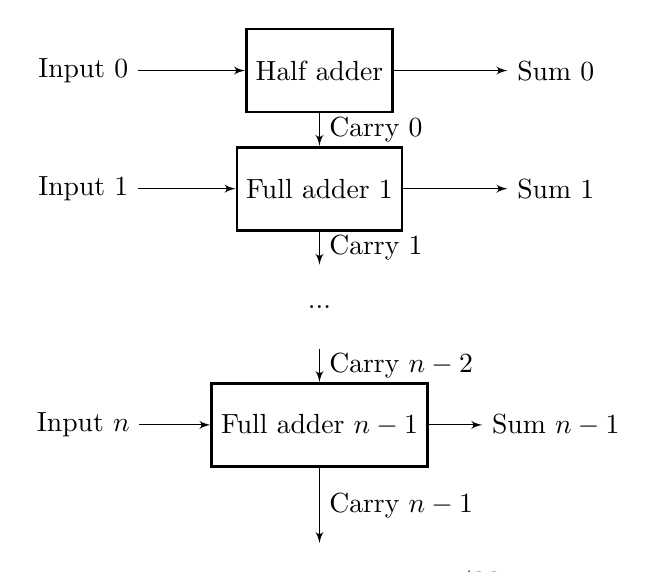
\begin{tikzpicture}[node distance=1.5cm]
        \node[block] (half) {Half adder};
        \node[block, below of=half] (full1) {Full adder 1};
        \node[empty, below of=full1] (dot) {...};
        \node[block, below of=dot] (fulln) {Full adder $n-1$};

        \node[empty, left of=half] (spacingl) {};
        \node[empty, right of=half] (spacingr) {};

        \node[empty, left of=spacingl] (in0) {Input 0};
        \node[empty, below of=in0] (in1) {Input 1};
        \node[empty, below of=in1] (vertspacel) {};
        \node[empty, below of=vertspacel] (inn) {Input $n$};

        \node[empty, right of=spacingr] (out0) {Sum 0};
        \node[empty, below of=out0] (out1) {Sum 1};
        \node[empty, below of=out1] (vertspacer) {};
        \node[empty, below of=vertspacer] (outn) {Sum $n-1$};
        \coordinate[below of=fulln] (carry);

        \path[draw, ->] (in0) -- (half);
        \path[draw, ->] (in1) -- (full1);
        \path[draw, ->] (inn) -- (fulln);

        \path[draw, ->] (half) -- (out0);
        \path[draw, ->] (full1) -- (out1);
        \path[draw, ->] (fulln) -- (outn);

        \path[draw, ->] (half) -- node [midway, right] {Carry 0} (full1);
        \path[draw, ->] (full1) -- node [midway, right] {Carry 1} (dot);
        \path[draw, ->] (dot) -- node [midway, right] {Carry $n-2$} (fulln);
        \path[draw, ->] (fulln) -- node [midway, right] {Carry $n-1$} (carry);
    \end{tikzpicture}
    \caption{An $n$-bit adder composed of a half adder, and $n-1$ full adders.
    Note: Input A and B are both inside the inputs for simplicity.}
    \label{fig:n-bit-adder}
\end{figure}

\subsubsection{Testing}
I have tested both the half adder and the full adder, by giving each every
possible input, and for each, compared them to their expected output. For the
$n$-bit adder, I have made a function, that takes an integer as input, sends it
along the corresponding input wires. I have also made a similar function, that
takes the values from the output wires and packs it into an integer. I start by
testing if it can make one of the simplest additions: 2+2. Then I check if it
can overflow, i.e. set the Carry $n-1$ to \texttt{1}. Finally, I run a series
of random numbers through the adder, and check if the output is the expected
sum of the two numbers.


%\newpage
\section{Core components}
\label{sec:components}
\subsection{Register file}
The register file is the component that holds values for the processor. It is
the first step in a memory hierarchy, and thus the fastest memory available.
There are 32 registers in a 32-bit MIPS processor. The registers are devided
into groups based on their usage. This does not matter from a hardware
perspective, except for register 0, which is immutable and always 0.

A register file has 5 inputs: Read address A, Read address B, Write enabled,
Write address and Write data. It also has two outputs: Output A and Output B.
We need to be careful of the order in which we read and write from the register
file. We need to make sure that when an instruction reads from the register
file, it always gets the latest data, i.e. if an instruction reads from the
same register as a previous instruction writes to, it should get the written
value. This is easy to fix in the single cycle processor, as we just need to
write before reading.

\begin{figure}
    \centering
    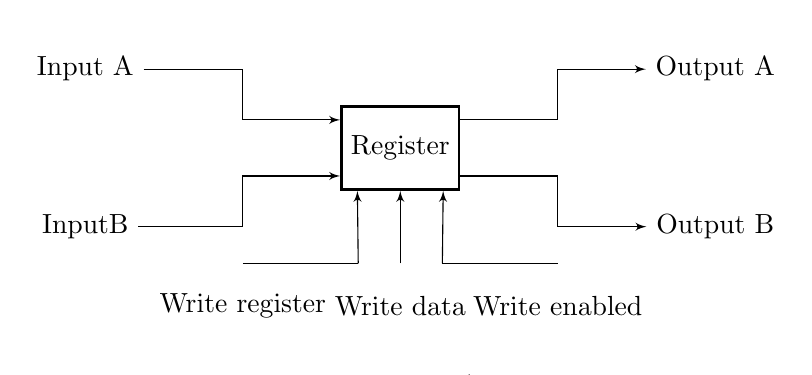
\begin{tikzpicture}[node distance=2cm]
        \node[empty] (inputa) {Input A};
        \node[empty, below of=inputa] (inputb) {InputB};

        \node[empty, right of=inputa] (spacing) at ($(inputa)!0.5!(inputb)$) {};
        \node[block, right of=spacing] (register) {Register};
        \node[empty, below of=register] (writedata) {Write data};
        \node[empty, left of=writedata] (write) {Write register};
        \node[empty, right of=writedata] (writeenabled) {Write enabled};

        \node[empty, right of=inputa] (space) {};
        \node[empty, right of=space] (spacee) {};
        \node[empty, right of=spacee] (spaceee) {};
        \node[empty, right of=spaceee] (outputa) {Output A};
        \node[empty, below of=outputa] (outputb) {Output B};
        \node[empty, left of=outputb] (bspace) {};

        \path[draw, -] (inputa) -| (spacing.north);
        \path[draw, ->] (spacing.north) |- (register.155);
        \path[draw, -] (inputb) -| (spacing.south);
        \path[draw, ->] (spacing.south) |- (register.205);

        \path[draw, -] (write) |- (writedata.135);
        \path[draw, ->] (writedata.135) -- (register.225);
        \path[draw, ->] (writedata) -- (register);
        \path[draw, -] (writeenabled) |- (writedata.45);
        \path[draw, ->] (writedata.45) -- (register.315);

        \path[draw, -] (register.335) -| (bspace.north);
        \path[draw, ->] (bspace.north) |- (outputb);
        \path[draw, -] (register.25) -| (spaceee.south);
        \path[draw, ->] (spaceee.south) |- (outputa);
    \end{tikzpicture}
    \caption{The register file}
    \label{fig:register}
\end{figure}

\bf{Testing} - I start by testing if some of the initial values of the register
file is correctly set to 0. Then I test if I can write to a register, and
whether or not I can read the same value from the same address in the register.
Then, I try to write to all of the registers, except for 0, and check whether
or not the output that I get, corresponds with the output that I wrote.

\subsection{ALU}
The ALU (Arithmetic Logic Unit) is the part of the processor, which makes the
actual computation. It takes three inputs: InputA, InputB and an ALU opcode
indicating which computation to perform. It has two outputs: The result of the
computation, and a zero flag indicating whether or not the result of the
computation was 0.

I follow the approach from the book % TODO ref!
and have implemented the basic processor operations: \texttt{add}, \texttt{sub},
\texttt{and}, \texttt{or} and \texttt{slt} (set less than).

I have tested each of the four operations.


%\newpage
\section{Single cycle MIPS processor}
\label{sec:single-cycle}
In this section, we will be combining the core components into a single cycle
MIPS processor, i.e. a processor where exactly one instruction is executed per
clock cycle. When it is in place, we will be writing the first program, and
compiling it into the processor, and running it.

Following the single cycle MIPS processor, we will be extending
the processor so that it can handle more instructions. Along each added
instruction, we will be extending our first program, in order to verify that
the instruction works.

Finally, we will be writing two programs, and look into compiling them into a
series of hex values, that we can copy straight into the Instruction Memory.

\subsection{Wiring up the processor}
\begin{figure}
    \centering
    \scalebox{0.5}{
        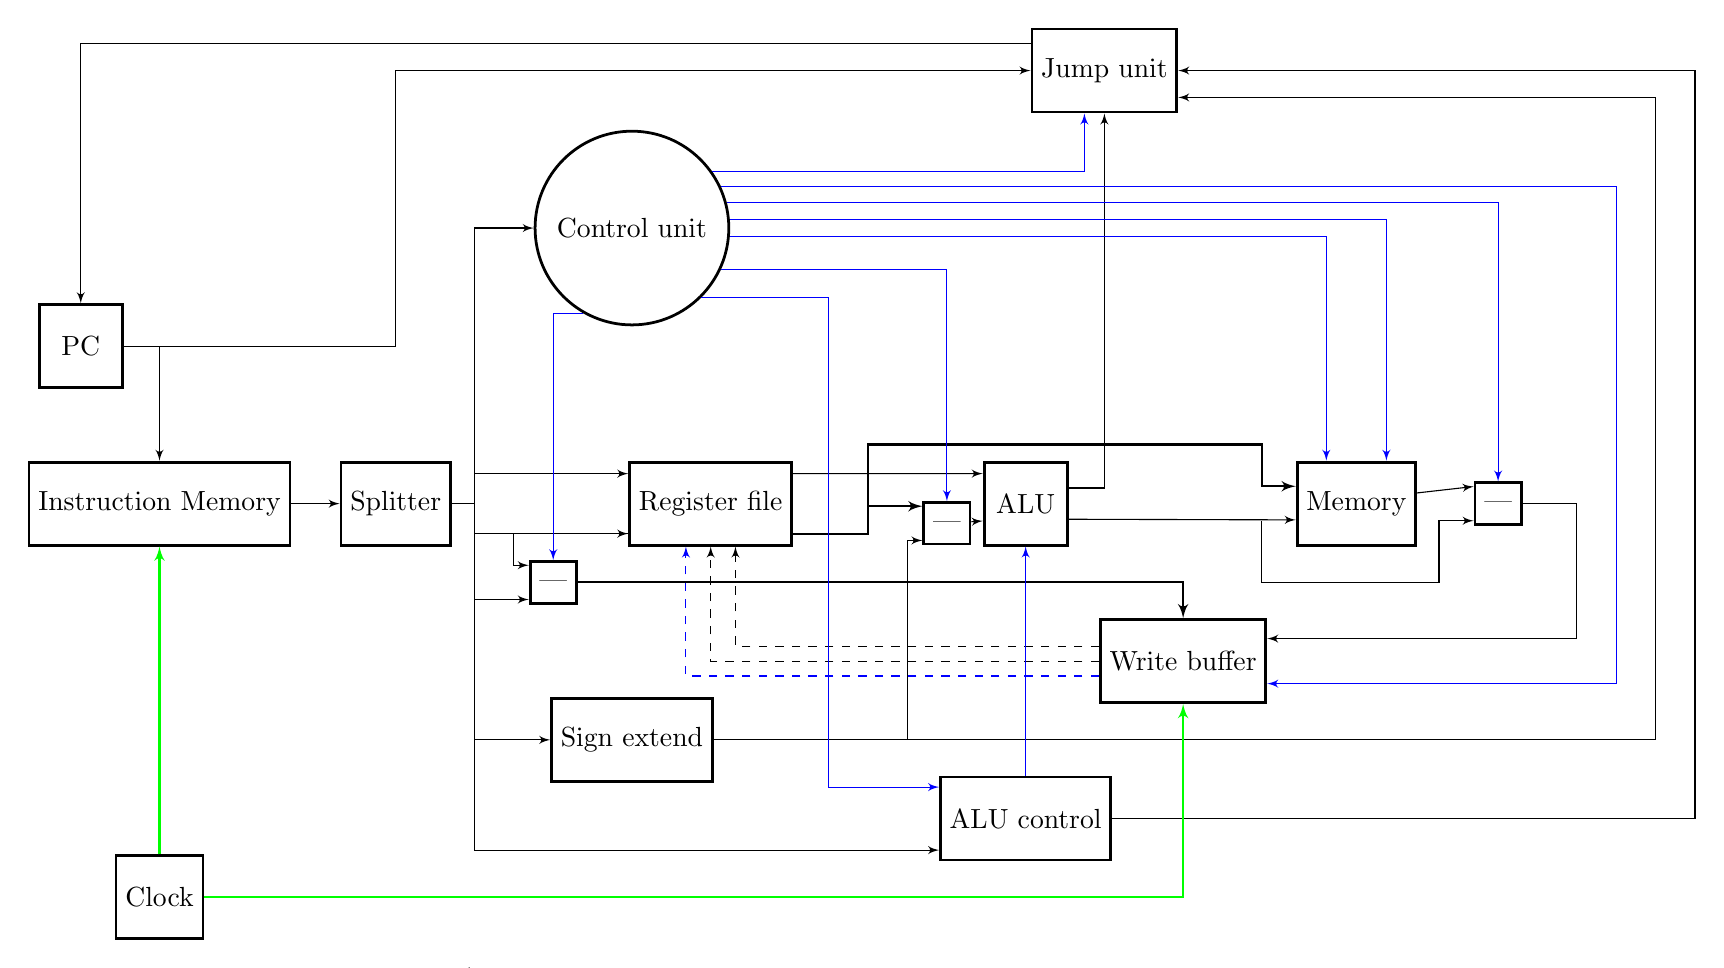
\begin{tikzpicture}
            \node[block] (reg) at (0,0) {Register file};
            \node[control] (cont) at (-1,3.5) {Control unit};
            \node[block] (jump) at (5,5.5) {Jump unit};
            \node[empty] (splitspace) at (-3,0) {};
            \node[block] (split) at (-4,0) {Splitter};
            \node[block] (if) at (-7,0) {Instruction Memory};
            \node[block] (sign) at (-1,-3) {Sign extend};
            \node[block] (alu) at (4,0) {ALU};
            \node[block] (alucont) at (4,-4) {ALU control};
            \node[block] (mem) at (8.2,0) {Memory};
            \node[mux] (memread) at (10,0) {|};
            \node[mux] (imm) at (3, -0.25) {|};
            \node[mux] (regdst) at (-2,-1) {|};
            \node[block] (pc) at (-8, 2) {PC};
            \node[block] (writebuf) at (6, -2) {Write buffer};

            \path[draw, ->] (if) -- (split);
            \path[draw, -] (split) -- (splitspace.center);
            \path[draw, ->] (splitspace.center) |- (sign);
            \path[draw, ->] (splitspace.center) |- (cont);
            \path[draw, ->] (splitspace.center) |- (reg.160);
            \path[draw, ->] (splitspace.center) |- (reg.200);
            \path[draw, ->] (splitspace.center) |- (alucont.200);
            \path[draw, ->] (splitspace.center) |- (regdst.215);
            \path[draw, ->] (reg.200) -| (-2.5, -0.5) |- (regdst.145);
            \path[draw, ->] (alucont) -| (12.5, 0) |- (jump);
            \path[draw, thick, ->] (reg.340) -| (2,-0.25) |- (imm.145);
            \path[draw, thick, ->] (2,-0.25) |- (3,0.75) -- (7,0.75) |-
            (mem.164);
            \path[draw, ->] (reg.20) -- (alu.145);
            \path[draw, ->] (alu.20) -| (jump);
            %\path[draw, ->] (alu.340) -- (jal);
            %\path[draw, ->] (jal) -- (mem.196);
            %\path[draw, ->] (jal) -- (writebuf);
            \path[draw, ->] (alu.340) -- (mem.195);
            \path[draw, ->] (imm) -- (alu.202);
            \path[draw, ->] (7, -0.22) |- (8, -1) -| (9.25,-0.5) |-
            (memread.215);
            \path[draw, ->] (mem.10) -- (memread.145);
            \path[draw, ->] (sign) -| (2.5, -1) |- (imm.215);
            \path[draw, ->] (2.5,-3) -| (12, 0) |- (jump.340);
            %\path[draw, thick, ->] (regdst) -| (5, -0.6) |- (jal.210);
            \path[draw, thick, ->] (regdst) -| (writebuf);
            \path[draw, ->] (pc) -| (if);
            \path[draw, ->] (pc) -| (-4, 4) |- (jump);
            \path[draw, ->] (jump.160) -| (pc);
            \path[draw, ->] (memread) -| (11, -1) |- (writebuf.15);
            \path[draw, dashed, ->] (writebuf.170) -| (reg.300);
            \path[draw, dashed, ->] (writebuf) -| (reg);
            \path[draw, dashed, ->, color=blue] (writebuf.190) -| (reg.240);

            \path[draw, ->, color=blue] (alucont) -- (alu);
            \path[draw, ->, color=blue] (cont.35) -| (jump.245);
            \path[draw, ->, color=blue] (cont.25) -| (11.5,0) |-
            (writebuf.345);
            \path[draw, ->, color=blue] (cont.15) -| (memread);
            \path[draw, ->, color=blue] (cont.5) -| (mem.55);
            \path[draw, ->, color=blue] (cont.355) -| (mem.125);
            \path[draw, ->, color=blue] (cont.335) -| (imm);
            \path[draw, ->, color=blue] (cont.315) -| (1.5, 0.5) |-
            (alucont.160);
            \path[draw, ->, color=blue] (cont.240) -| (regdst);

            \node[block] (clock) at (-7, -5) {Clock};
            \path[draw, ->, thick, color=green] (clock) -- (if);
            \path[draw, ->, thick, color=green] (clock) -| (writebuf);
        \end{tikzpicture}
    }
    \caption{Simple single cycle MIPS processor. The units with | indicate
    multiplexors}
    \label{fig:simple-full}
\end{figure}

\begin{figure}
    \centering
    \scalebox{0.5}{
        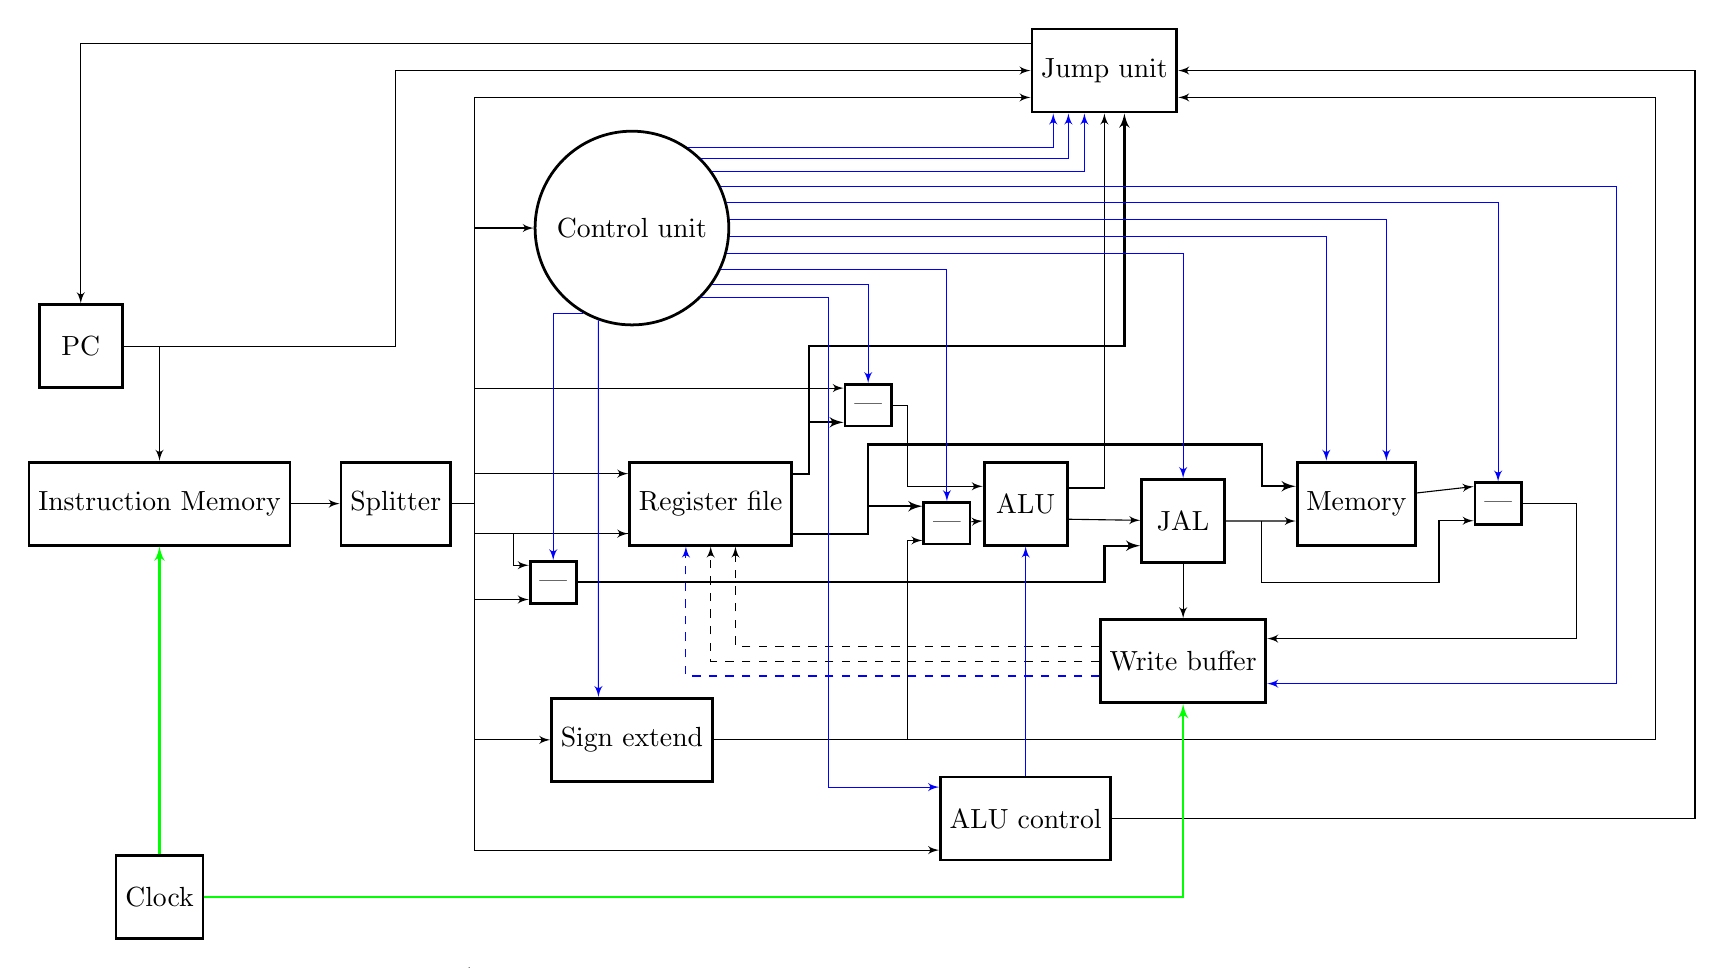
\begin{tikzpicture}
            \node[block] (reg) at (0,0) {Register file};
            \node[control] (cont) at (-1,3.5) {Control unit};
            \node[block] (jump) at (5,5.5) {Jump unit};
            \node[empty] (splitspace) at (-3,0) {};
            \node[block] (split) at (-4,0) {Splitter};
            \node[block] (if) at (-7,0) {Instruction Memory};
            \node[block] (sign) at (-1,-3) {Sign extend};
            \node[block] (alu) at (4,0) {ALU};
            \node[block] (alucont) at (4,-4) {ALU control};
            \node[block] (mem) at (8.2,0) {Memory};
            \node[block] (jal) at (6,-0.22) {JAL};
            \node[mux] (memread) at (10,0) {|};
            \node[mux] (shmt) at (2,1.25) {|};
            \node[mux] (imm) at (3, -0.25) {|};
            \node[mux] (regdst) at (-2,-1) {|};
            \node[block] (pc) at (-8, 2) {PC};
            \node[block] (writebuf) at (6, -2) {Write buffer};

            \path[draw, ->] (if) -- (split);
            \path[draw, -] (split) -- (splitspace.center);
            \path[draw, ->] (splitspace.center) |- (sign);
            \path[draw, ->] (splitspace.center) |- (cont);
            \path[draw, ->] (splitspace.center) |- (reg.160);
            \path[draw, ->] (splitspace.center) |- (reg.200);
            \path[draw, ->] (splitspace.center) |- (jump.200);
            \path[draw, ->] (splitspace.center) |- (alucont.200);
            \path[draw, ->] (splitspace.center) |- (regdst.215);
            \path[draw, ->] (splitspace.center) |- (shmt.145);
            \path[draw, ->] (reg.200) -| (-2.5, -0.5) |- (regdst.145);
            \path[draw, ->] (alucont) -| (12.5, 0) |- (jump);
            \path[draw, thick, ->] (reg.340) -| (2,-0.25) |- (imm.145);
            \path[draw, thick, ->] (2,-0.25) |- (3,0.75) -- (7,0.75) |-
            (mem.164);
            \path[draw, thick, ->] (reg.20) -| (1.25,0.5) |- (shmt.215);
            \path[draw, thick, -] (1.25,0.5) |- (4,2);
            \path[draw, thick, ->] (4,2) -| (jump.295);
            \path[draw, ->] (shmt) -| (2.5, 0.5) |- (alu.158);
            \path[draw, ->] (alu.20) -| (jump);
            \path[draw, ->] (alu.340) -- (jal);
            \path[draw, ->] (jal) -- (mem.196);
            \path[draw, ->] (imm) -- (alu.202);
            \path[draw, ->] (7, -0.22) |- (8, -1) -| (9.25,-0.5) |-
            (memread.215);
            \path[draw, ->] (mem.10) -- (memread.145);
            \path[draw, ->] (sign) -| (2.5, -1) |- (imm.215);
            \path[draw, ->] (2.5,-3) -| (12, 0) |- (jump.340);
            \path[draw, thick, ->] (regdst) -| (5, -0.6) |- (jal.210);
            \path[draw, ->] (pc) -| (if);
            \path[draw, ->] (pc) -| (-4, 4) |- (jump);
            \path[draw, ->] (jump.160) -| (pc);
            \path[draw, ->] (jal) -- (writebuf);
            \path[draw, ->] (memread) -| (11, -1) |- (writebuf.15);
            \path[draw, dashed, ->] (writebuf.170) -| (reg.300);
            \path[draw, dashed, ->] (writebuf) -| (reg);
            \path[draw, dashed, ->, color=blue] (writebuf.190) -| (reg.240);

            \path[draw, ->, color=blue] (alucont) -- (alu);
            \path[draw, ->, color=blue] (cont.55) -| (jump.220);
            \path[draw, ->, color=blue] (cont.45) -| (jump.230);
            \path[draw, ->, color=blue] (cont.35) -| (jump.245);
            \path[draw, ->, color=blue] (cont.25) -| (11.5,0) |-
            (writebuf.345);
            \path[draw, ->, color=blue] (cont.15) -| (memread);
            \path[draw, ->, color=blue] (cont.5) -| (mem.55);
            \path[draw, ->, color=blue] (cont.355) -| (mem.125);
            \path[draw, ->, color=blue] (cont.345) -| (jal);
            \path[draw, ->, color=blue] (cont.335) -| (imm);
            \path[draw, ->, color=blue] (cont.325) -| (shmt);
            \path[draw, ->, color=blue] (cont.315) -| (1.5, 0.5) |-
            (alucont.160);
            \path[draw, ->, color=blue] (cont.250) -- (sign.128);
            \path[draw, ->, color=blue] (cont.240) -| (regdst);

            \node[block] (clock) at (-7, -5) {Clock};
            \path[draw, ->, thick, color=green] (clock) -- (if);
            \path[draw, ->, thick, color=green] (clock) -| (writebuf);
        \end{tikzpicture}
    }
    \caption{Full single cycle MIPS processor. The units with | indicate
    multiplexors. Black wires indicate data wires. Blue wires indicate control
    wires. Green wires indicate clock}
    \label{fig:full}
\end{figure}


%    \item[Jump] Controls whether or not the instruction is a jump instruction,
%        i.e. if the \texttt{PC} register should be changed.

%    \item[JAL] Contrals whether or not the instruction is a \texttt{jal}
%        instruction, i.e. that the \texttt{PC+4} address should be stored.

%    \item[LogicalImmediate] Controls whether or not the sign extender should
%        be a sign extender, in the case of a numeral immediate, or if it
%        should be a zero extender, in the case of a logical I-format
%        instruction.

%\subsection{Jump control}
%The jump control is the part of the processor, that based on the instruction
%changes the value of the PC register. There are two ways to jump: by branching
%and by jumping.
%
%\subsubsection*{Implementation}
%We start by implementing the control for the branching logic. We need to
%support 2 branch instructions in our basic processor: branch equal and branch
%not equal. Therefore we will need two signals: \texttt{Branch} and
%\texttt{BranchNot}. The \texttt{Branch} is used to indicate that the
%instruction should change the PC register. The \texttt{BranchNot} is used to
%choose whether or not the \texttt{Zero} flag from the ALU should be
%\texttt{1} or \texttt{0} for the instruction to branch. In both instructions,
%we compute the subtraction of the two input registers, and if the result is
%\texttt{1} they are equal, otherwise they are not equal. The \texttt{Zero}
%signal is then send to an \texttt{AND} gate along with the \texttt{Branch}
%signal.
%
%Then we need to implement the jump unit. This is a little bit easier, as we do
%not depend on anything from the ALU. The problem is that we need to change the
%decoder to accept a new format: the J-format. The J-format consists of an
%opcode, and a 26-bit address. The address is left shifted by 2, to ensure word
%alignment, and the upper 4 bits of the PC is added to the final address. We
%also need another control signal: \texttt{Jump}. We use this to multiplex
%between the newly computed address and the output from the previous mux (branch
%or pc+4).
%
%\subsubsection*{Testing}
%We test the jump unit by adding jump instructions in the program within the
%Instruction Memory.

%\subsection{Adding additional instructions}
%To add additional instructions, we need to add additional circuitry and entries
%in the \tt{enum}s. We will go through implementing the MIPS core instruction
%set.
%
%We start with the remaining R format instructions (Except for shifting,
%multiplication and division). This is straightforward, as we only need to add
%additional entries to the \tt{enum}s, add the additional cases in the
%\tt{switch} in the ALU control and in the \tt{switch} in the ALU.
%
%For shifting, we need to extract extra information from the instruction in the
%Splitter: the \tt{shamt} field. Following this, we add an additional control
%signal, and multiplex on whether it should be the value read from the registers
%or the \tt{shamt}, which should be the B input for the ALU.
%
%Then we have the remaining arithmetic I format instructions. This is also
%straightforward, as we only need to extend the \tt{enum}s, and add additional
%entries to the \tt{switch} in the ALU control.
%
%Next we need the \tt{jal} instruction. Here we need circuitry to store the
%contents of the \tt{PC} register. To do this, we send the \tt{PC} to the
%\tt{EX} stage, and multiplex on the output from the ALU and the \tt{PC}, with
%the \tt{JAL} control signal.
%
%Next we need the \tt{jr} instruction. We add an additional signal, and
%multiplex on the value read from register, and the normal \tt{PC+4}.
%
%Then we have the \tt{mult}, \tt{multu}, \tt{div} and \tt{divu} instructions.
%These are all R format, so we follow the same procedure. However, instead of
%sending the result on the ALU result bus, we store it in two additional
%registers, which we keep in the ALU: \tt{HI} and \tt{LO}. Following this, we
%can also easily add the instructions \tt{mfhi}, \tt{mflo}, \tt{mthi} and
%\tt{mtlo}, which moves data to and from the two new registers.
%
%Finally, we have the \tt{bne} instruction. We add an additional signal, and
%multiplex the \tt{NOT}ed \tt{zero} signal from the ALU as the signal for the
%branching \tt{AND} gate.
%
%\subsection{Test programs}
%Snak om at bruge MARS!
%
%Now that we have our single cycle MIPS processor, we are ready to throw actual
%instructions at it. We start by collecting all of the smaller test instructions
%into a full test program. SE APPENDIX! (og lav det for den sags skyld)
%
%Then we have a Quicksort written in MIPS assembly.


%\newpage
\section{Pipelining}
\label{sec:pipelining}
In this section, we will be looking at pipelining our single cycle MIPS
processor, and handle the problems, which are introduced by pipelining.

We start by going through the background and motivation for pipelining, and
then proceed on how to extend our single cycle MIPS processor to have pipes.

As mentioned, pipelining introduces new problems to handle in the processor,
and we will solve it by adding two new components: the forwarding unit, which
forwards results from previous instructions to later instructions, and the
hazard detection unit, which controls when to stall the pipeline, and when the
instruction should read the forwarded value, or the value stored in the
Register File.

Throughout each step, we will also be writing programs, in order to verify that
our processor behaves as specified.

\subsection{Introducing the pipes}


\subsection{Forwarding}
\subsection{Hazard Detection}


%\newpage
\section{Transpiling and synthesizing SME}
\label{sec:synthesis}
In this section, I will be describing the steps required to implement an SME
network onto an actual FPGA. I start with the initial Logic Gates design, as it
is very simple to verify and because it does not have any requirements
regarding clocking.

Then I will be implementing the single cycle MIPS processor and finally show
how to communicate with the hardware implemented on the FPGA. This section will
be very hardware specific, as I have not verified or developed a
general approach, which will run on additional hardware.

All of the source code, both for SME and VHDL, can be found
at~\cite{ref:github}.

\subsection{General workflow}
This section will give a general description of the workflow required for
implementing hardware on an FPGA using SME. A short overview of the steps and
their order, can be seen in Figure~\ref{fig:general-workflow},

\begin{figure}
    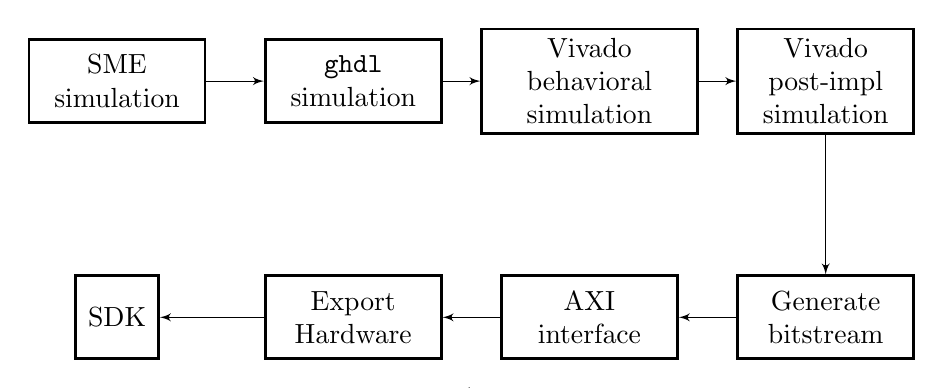
\begin{tikzpicture}[node distance=3cm]
        \node[block, text width=2cm, align=center] (sme) {SME\\simulation};
        \node[block, right of=sme, text width=2cm, align=center] (ghdl) {\texttt{ghdl}\\simulation};
        \node[block, right of=ghdl, text width=2.5cm, align=center] (behav) {Vivado\\behavioral\\simulation};
        \node[block, text width=2cm, align=center, right of=behav] (post) {Vivado\\post-impl\\simulation};
        \node[block, below of=post, text width=2cm, align=center] (bitstream) {Generate\\bitstream};
        \node[block, left of=bitstream, text width=2cm, align=center] (interface) {AXI\\interface};
        \node[block, left of=interface, text width=2cm, align=center] (export) {Export\\Hardware};
        \node[block, left of=export] (sdk) {SDK};

        \path[draw, ->] (sme) -- (ghdl);
        \path[draw, ->] (ghdl) -- (behav);
        \path[draw, ->] (behav) -- (post);
        \path[draw, ->] (post) -- (bitstream);
        \path[draw, ->] (bitstream) -- (interface);
        \path[draw, ->] (interface) -- (export);
        \path[draw, ->] (export) -- (sdk);
    \end{tikzpicture}
    \caption{The general workflow for construction actual hardware using SME.}
    \label{fig:general-workflow}
\end{figure}
In order to implement hardware onto an FPGA, one must describe the hardware
using a hardware description language such as VHDL or Verilog. As mentioned
before, SME can be transpiled into VHDL and as such provides a high level
approach for hardware design. Therefore, the first thing to do is to write an
SME network, verify that it runs as expected, and then checking that the
transpiler does not fail to transpile. The top-level input and output busses has
to be specified in SME. A top-level bus is a bus going either in or out of the
SME network.

To generate VHDL from SME, the \texttt{Main()} function needs two additional
lines: \texttt{.BuildCSVFile()} and \texttt{.BuildVHDL()}
\begin{lstlisting}
public static void Main(string[] args)
{
    new Simulation()
        .BuildCSVFile()
        .BuildVHDL()
        .Run(typeof(MainClass).Assembly);
}
\end{lstlisting}
This will generate the VHDL code, a testbench for the VHDL code and a
\texttt{csv} trace file used by the testbench. The trace file contains all the
values sent on all of the busses within the network during simulation. The
testbench takes all the input values in the \texttt{csv} file, sends them along
the input busses, and finally verifies that the values on the other busses
matches the value stored in the \texttt{csv} file.

Once the VHDL has been generated, the VHDL can be verified by using
\texttt{ghdl}~\cite{ref:ghdl}. \texttt{ghdl} is an commandline simulator for
VHDL. SME provides a testbench and a \texttt{Makefile} for running the
testbench using \texttt{ghdl}. As such, to verify the generated VHDL, one only
needs to run \texttt{make} inside the output \texttt{vhdl/} folder.

Once the \texttt{ghdl} simulation has been passed, the VHDL files can be
imported into a project in Vivado~\cite{ref:vivado}. Vivado is a development
environment created by Xilinx, an FPGA vendor, for designing and implementing
hardware on an FPGA.  When creating the project, Vivado needs to know the
target FPGA. In this project, I have been using a ZedBoard.

A ZedBoard is a development board, which contains a Xilinx Zynq system on chip.
A Zynq chip has two parts: a processing system (an ARM processor) and
programmable logic (FPGA). These two parts are connected in two places: through
an AXI interconnect and through DDR memory.  I will be using the AXI
interconnect, when communicating with the FPGA.  AXI (Advanced eXtensible
Interface)~\cite{ref:axi} is an interconnect specification, which communicates
by using transactions. I am not going to focus on the details of the protocol.
Additionally, the ZedBoard comes with a few buttons, switches and LEDs, which
are connected to the FPGA part of the Zynq chip.  These buttons and LEDs can be
used as easy to set up input/output.

Once the project have been created in Vivado, the behavorial simulation should
be run. The behavorial simulation is the same as the \texttt{ghdl} simulation
and should as such produce the same result.

Then the design should be elaborated into Register Transfer Level (RTL). RTL is
a design abstraction, which consists of lower level components (E.g. gates and
registers) wired together. The RTL schematic can also be used to verify whether
or not the design interpreted by Vivado matches the SME network. The schematic
shows all of the top-level input and output busses. Additionally, there are the
\texttt{CLK} (clock) and \texttt{RST} (reset) busses. The \texttt{CLK} bus is
the clock signal used throughout the network.  The \texttt{RST} bus is the
reset signal. All the SME processes uses the \texttt{RST} signal, but only the
clocked processes uses the \texttt{CLK} signal.

Within the RTL, the top-level input and output busses has to be connected to
some specified wire on the FPGA (E.g. input signal from a button). At the same
time, the communication standard should be specified. I just choose the
default, as I do not have any special requirements. This is also where the
clock signal and the reset signal are connected to wires. All of this is
required by Vivado, in order for it to place and route the design.

Then the project is ready to be synthesized, placed and routed. This is done by
the click of a button in Vivado and takes quite some time, especially for
larger projects.

If the design uses a clock signal (i.e. has clocked processes), the first step
is to synthesize the design. This is due to once the design have been
synthesized, clocking constraints can be introduced. Vivado uses these
constraints as a target, when it is placing and routing the synthesized design.
The only clocking constraint for the designs in this thesis is the clockrate.
When Vivado has placed and routed the design, it creates a timing report,
stating whether or not the timing constraints where met. The timing report
computes a slack on each of the paths in the implementation. Slack is the
difference on how long it takes the signal to traverse a path, compared to the
clocrate constraint. E.g. if it takes a signal 13 nanoseconds to traverse a
path and the clockrate is specified to 10 nanoseconds per clock cycle, then the
slack will be -3 nanoseconds. If the slack is positive, the clockrate should be
increased. If the slack is negative, the clockrate should be reduced.  After
the clocking constraints have been introduced, the project needs to be
synthesized again.

Once the project have been placed and routed, the post-implementation timing
simulation should be run. This simulation is the closest to actual hardware, as
it models all of the components of the FPGA, all the wires and the timing on
the wires. As such, this is a very heavy simulation and takes some time to run.

Furthermore, in the implemented design, Vivado can produce some interesting
reports. The first interesting report is the utilization report, which reports
how much of the logic available on the target board have been used. Generally,
the most interesting metrics in the report are: Logic, IO, Registers, Block
Memory and MMCM (clock multiplier/divider). In theory, the utilization report
can be used to see how many instances of a design the target board can hold, by
taking 100 divided by the metric with the highest value. E.g. the Single Cycle
processor has Logic as the highest usage at 17\% on the ZedBoard. I.e.
$100/17=5.88\approx5$ cores could be fitted onto the ZedBoard.

Then we have the Power report, which reports an estimate of the power
consumption of the design. The report contains a lot of metrics, but the one I
focus on is the dynamic power consumption. This is the sum of approximate power
consumption of each of the implemented components on the FPGA. I.e. the
approximate power consumption of the implemented design.

The final report is the timing summary, which I will describe later.

If the post-implementation simulation passes, it should also work as expected
on actual hardware. If clocking constraints were needed, the clock signal
should be modified to match the clocking constraints. In order to do this, the
design have to be implemented in a block design. There is a problem with the
transpiled VHDL from SME. The top module uses custom types and Vivado does not
allow custom types in a block design. To solve this, all the custom types must
be changed to be standard types. E.g. \texttt{T\_SYSTEM\_UINT32} becomes
\texttt{std\_logic\_vector(31 downto 0)}. Once this have been changed, the top
module can be inserted into a block design. The clocking wizard should be
added, in order to modify the clock to match the clocking constraints. Once the
block design have been constructed, it should be made into a HDL wrapper, such
that it can be synthesized, placed and routed. The final step is to generate
the bitstream and write it to the FPGA.

Once the running bitstream has been verified, it is time to communicate with
it. To do this, I must construct a custom Intellectual Property (IP). An IP is
an already verified hardware component, which can have standardized connection
and with these be connected to other IPs in a block design. This custom IP
should have an AXI interface, so it can communicate with the ARM processor on
the Zynq chip.

Vivado provides a template for generating IPs with an AXI interfaces. This
template uses registers to send and receive information trough the interface. So
before where the top-level busses were connected to wires on the FPGA, they must
now be connected to these registers. This is done in VHDL, as the current
version of SME does not support this. I could have written the AXI interface as
an SME process. Doing it by VHDL seemed simpler however.

Once the IP have been constructed and verified, a new project with a new block
design should be added. Inside the block design, the processing system of the
Zynq chip should be added and connected to the custom IP with the AXI interface.
Additionally, if timing constraints on the clock was needed during the
implementation of before constructing the IP, then the clocking
wizard should be added to the block design in order to either multiplying or
dividing the clock. Again, once the block design have been verified, it should
be made into a synthesizable component, by creating a HDL wrapper.

Once the bitstream has been generated, the hardware should be exported and
opened in the Xilinx SDK. From here, the ARM processor on the Zynq chip can be
programmed bare-metal. Bare-metal programming is programming without an
operating system, i.e. injecting the compiled machine code directly into the
instruction cache of the ARM processor. The AXI interface have received a
memory address, and the SDK should contains library with functions for
accessing the registers through the AXI interface. With this, a driver should
be written for the new logic.

Once the driver has been written, I can interface with the FPGA on the Zynq
chip, by programming the ARM processor.

\subsection{Logic gates}
I start by implementing the first SME network, which I constructed: the logic
gates. This network consisted of five SME processes: the four gates and the
tester process. The tester process was only used for verification purposes, and
should not be present in the generated VHDL. To solve this, the tester process
should not be a \texttt{ClockedProcess}, but rather a
\texttt{SimulatedProcess}. A \texttt{SimulatedProcess} has the same behavior as
the \texttt{ClockedProcess}, except it does not generate any VHDL. The value
which it inputs and outputs are caputered in the CSV tracefile, which is used
by the generated testbench. Furthemore, all of the inputs and outputs to the
gates, should be made top-level.

When running the testbench trough \texttt{ghdl}, I get the following
output:
\begin{lstlisting}
TestBench_LogicGates.vhdl:166:8:@50ns:(report note): completed after 5 clockcycles
\end{lstlisting}
Which states that the simulation ran as expected in 5 clockcycles.

Then I create the Vivado project. As mentioned in the general workflow,
the next step is to run the behavorial simulation and verify that it
runs as expected. Running the Logic Gates should produce the waveform seen in
Figure~\ref{fig:logic-wave}.

\begin{figure}
    \includegraphics[width=\linewidth]{logic_gates_wave}
    \caption{The waveform of the Logic Gates simulation.}
    \label{fig:logic-wave}
\end{figure}

Then I verify that the RTL schematic matches the SME network. The RTL
network of the Logic Gates project can be seen in Figure~\ref{fig:logic-rtl}
and it matches the structure in Figure~\ref{fig:logic-test}.

\begin{figure}
    \includegraphics[width=\linewidth]{logic_gates_rtl}
    \caption{The RTL schematic of the Logic Gates project.}
    \label{fig:logic-rtl}
\end{figure}

Then I choose where the top-level input and output wires should be
connected. On the ZedBoard, I connect the outputs to the LEDs and the
inputs to the switch buttons. I wire the reset signal to a button. Since the
Logic Gates project does not use the clock, anything can be connected.

The next step is to synthesize, place and route the project. Once it is done,
the post-implementation simulation is run. The waveform that it produces, is the
same as Figure~\ref{fig:logic-wave}. The implemented design has a maximum
utilization of 4\%, which is the IO. It has an approximate power consumption of
0.001 watts. The comparison to the reported values of the other implementations
can be seen in Table~\ref{tab:impl-comp}.

Then the bitstream is generated and written to the ZedBoard. Flipping the
switches makes the LEDs light as shown in Figure~\ref{fig:logic-fpga}.

\begin{figure}
    \includegraphics[width=.24\textwidth]{FF2}
    \includegraphics[width=.24\textwidth]{FT2}
    \includegraphics[width=.24\textwidth]{TF2}
    \includegraphics[width=.24\textwidth]{TT2}
    \caption{The LEDs with the different configurations of flip switches on the
    ZedBoard. From left to right the inputs on each of the images are:
    false-false, false-true, true-false, true-true. The four LEDs from left to
    right on each image are: \texttt{AND}, \texttt{OR}, \texttt{NOT} and
    \texttt{XOR}. Note: \texttt{NOT} only considers the first input.}
    \label{fig:logic-fpga}
\end{figure}

Then the AXI interface is set up. This is done by creating a new project in
Vivado and within that create and package a new IP. In order to use the AXI
template that Vivado offers, I need to state how many registers it should have.
Since the Logic Gates project has two inputs and four outputs, I choose six
registers.

The AXI template creates two files. The first file contains a wrapper
component, which connects external connections to the inner components of the
IP. If I needed a clock signal or reset signal, which should be seperate from
the AXI clock and reset, the ports should be added here. The second file is the
registers component of the AXI interface, which handles reading and writing to
and from the slave registers.  I am going to extend the registers to have
signals from the Logic Gates and then extend the wrapper component, such that
the Logic Gates are connected to the registers component.

The registers component gets two new output signals: \texttt{bit1} and
\texttt{bit2}, and four new input signals: \texttt{and}, \texttt{or},
\texttt{not} and \texttt{xor}.
\begin{lstlisting}
-- Users to add ports here
bit1 : out std_logic;
bit2 : out std_logic;

andgate : in std_logic;
orgate  : in std_logic;
notgate : in std_logic;
xorgate : in std_logic;
-- User ports ends
\end{lstlisting}
I need to ensure that the slave registers that the Logic Gates writes to
are exclusively to the Logic Gates. I use slave registers 0 and 1 as the
input bits, and slave registers 2, 3, 4 and 5 as the output. As such, all the
occurrences where the registers component writes to slave registers 2, 3, 4 and 5,
are commented out.
\begin{lstlisting}
Before:
-- slave registor 2
slv_reg2(byte_index*8+7 downto byte_index*8) <= S_AXI_WDATA(byte_index*8+7 downto byte_index*8);

After:
-- slave registor 2
-- slv_reg2(byte_index*8+7 downto byte_index*8) <= S_AXI_WDATA(byte_index*8+7 downto byte_index*8);
\end{lstlisting}
Finally, the registers component needs the new logic. It outputs the contents of slave registers 0 and 1 to the \texttt{bit1} and
\texttt{bit2} busses. Then it should take the values from the four Logic Gate
outputs, and store them in slave registers 2, 3, 4 and 5:
\begin{lstlisting}
-- Add user logic here
bit1 <= slv_reg0(0);
bit2 <= slv_reg1(0);
slv_reg2(0) <= andgate;
slv_reg3(0) <= orgate;
slv_reg4(0) <= notgate;
slv_reg5(0) <= xorgate;
-- User logic ends
\end{lstlisting}
Then I need to extend the wrapper component. I start by adding the types
generated by SME:
\begin{lstlisting}
-- library SYSTEM_TYPES;
use work.SYSTEM_TYPES.ALL;

-- library CUSTOM_TYPES;
use work.CUSTOM_TYPES.ALL;
\end{lstlisting}
Then, I extend the component definition of the registers component to have
the added ports:
\begin{lstlisting}
port (
    bit1 : out std_logic;
    bit2 : out std_logic;
    andgate : in std_logic;
    orgate  : in std_logic;
    notgate : in std_logic;
    xorgate : in std_logic;
    S_AXI_ACLK  : in std_logic;
\end{lstlisting}
Then I add the component definition of the Logic Gates project, along with
the signals going from the Logic Gates to the registers component. For the
ports in the component definition, I add the ports specified in the SME
generated top-level file:
\newpage
\begin{lstlisting}
component LogicGates_export is
    port(

    -- Top-level bus Input signals
    Input_bit1: in T_SYSTEM_BOOL;
    Input_bit2: in T_SYSTEM_BOOL;

    -- Top-level bus Output signals
    Output_And: out T_SYSTEM_BOOL;
    Output_Or: out T_SYSTEM_BOOL;
    Output_Not: out T_SYSTEM_BOOL;
    Output_Xor: out T_SYSTEM_BOOL;


    -- User defined signals here
    -- #### USER-DATA-ENTITYSIGNALS-START
    -- #### USER-DATA-ENTITYSIGNALS-END

    -- Reset signal
    RST : in Std_logic;

    -- Clock signal
    CLK : in Std_logic
  );
end component LogicGates_export;
signal bit1 : std_logic;
signal bit2 : std_logic;

signal gates_and : std_logic;
signal gates_or  : std_logic;
signal gates_not : std_logic;
signal gates_xor : std_logic;
\end{lstlisting}
Then I map the signals to the instantiation of the registers component
\begin{lstlisting}
port map (
    bit1 => bit1,
    bit2 => bit2,
    andgate => gates_and,
    orgate  => gates_or,
    notgate => gates_not,
    xorgate => gates_xor,
    S_AXI_ACLK  => s00_axi_aclk,
\end{lstlisting}
Finally, the Logic Gates component needs to be instantiated. The clock and reset
signals uses the AXI clock and reset. Note: the AXI reset signal is
inverted compared to the signal expected by the SME generated code. I.e. AXI
resets when the signal is \texttt{0} and SME resets when the signal is
\texttt{1}.
\newpage
\begin{lstlisting}
-- Add user logic here
LogicGates_inst : LogicGates_export
port map (
    Input_bit1 => bit1,
    Input_bit2 => bit2,
    Output_And => gates_and,
    Output_Or  => gates_or,
    Output_Not => gates_not,
    Output_Xor => gates_xor,
    RST => s00_axi_aresetn,
    CLK => s00_axi_aclk
);
-- User logic ends
\end{lstlisting}
Now the Logic Gates project have been wrapped in an AXI interface. The RTL
schematic can be seen in Figure~\ref{fig:logic-axi-rtl}.
\begin{figure}
    \includegraphics[width=\linewidth]{logic_axi_rtl}
    \caption{The RTL schematic of the Logic Gates with AXI interface.}
    \label{fig:logic-axi-rtl}
\end{figure}
Then I package the IP, which is then available in the IP
catalog. In the original project, I create a block design. It needs
two components: the processing system and the Logic Gates with AXI interface. Upon
adding the processing system, Vivado gives the option to run block and
connection automation. The complete block design can be seen in
Figure~\ref{fig:logic-axi-block}.
\begin{figure}
    \includegraphics[width=\linewidth]{logic_axi_block}
    \caption{The finished block design contaning the processing system and the
    Logic Gates AXI IPs.}
    \label{fig:logic-axi-block}
\end{figure}
The next step is to create a HDL wrapper from the block design, and then
generate the bitstream. The custom types has to be added to the project,
otherwise the IP cannot be synthesized, as it cannot recognize the types. When
the bitstream has been generated, the hardware is exported to the Xilinx SDK.
Note: the bitstream must be included. The implemented Logic Gates with an AXI
interface has a maximum  utilization of 1\%, which is the Logic. It has an
approximate power consumption of 1.535 watts. This however, is due to the ARM
processor, which uses 1.529 watts. I.e. the Logic Gates with the AXI interface
has an approximate power consumption of $1.535-1.529=0.006$ Watts. The
comparison to the reported values of the other implementations can be seen in
Table~\ref{tab:impl-comp}.

In the SDK, I create a new Application project. I choose the
"Hello World" example project, and call it "Tester". The new code is added to
\texttt{Tester/src/helloworld.c}.

Creating the sample project will also create a Board Support Package (BSP)
called "Tester\_bsp". This BSP contains all the files related to the exported
hardware. The file I am most interested in is \texttt{Tester\_bsp/ps7\_cortex9
\_0/libsrc/LogicGates\_AXI\_v1\_0/src/LogicGates\_AXI.h}. This file contains
all the functions for reading and writing to the AXI registers. I also need
\texttt{xparameters.h}, as it contains the base address for the AXI interface.
Finally, I also need \texttt{xil\_io.h} as it contains the types returned byt
he read and write functions.
\begin{lstlisting}
#include "xparameters.h"
#include "LogicGates_AXI.h"
#include "xil_io.h"
\end{lstlisting}
Now, the default names given by Vivado and the SDK are a bit long and the
registers are numbered. Therefore, I give them shorter and more appropriate
names
\begin{lstlisting}
int base = XPAR_LOGICGATES_AXI_0_S00_AXI_BASEADDR;
int bit1 = LOGICGATES_AXI_S00_AXI_SLV_REG0_OFFSET;
int bit2 = LOGICGATES_AXI_S00_AXI_SLV_REG1_OFFSET;
int and = LOGICGATES_AXI_S00_AXI_SLV_REG2_OFFSET;
int or  = LOGICGATES_AXI_S00_AXI_SLV_REG3_OFFSET;
int not = LOGICGATES_AXI_S00_AXI_SLV_REG4_OFFSET;
int xor = LOGICGATES_AXI_S00_AXI_SLV_REG5_OFFSET;
\end{lstlisting}
To verify the hardware, I write all combinations of inputs to the registers, and verify that it
outputs the same as the truth table specified in Table~\ref{tab:truth-table}. I
write two functions: one for writing to the two input registers and one for
printing all of the registers.
\begin{lstlisting}
void print_regs() {
    xil_printf("%d %d | %d %d %d %d\n",
            LOGICGATES_AXI_mReadReg(base, bit1),
            LOGICGATES_AXI_mReadReg(base, bit2),
            LOGICGATES_AXI_mReadReg(base, and),
            LOGICGATES_AXI_mReadReg(base, or),
            LOGICGATES_AXI_mReadReg(base, not),
            LOGICGATES_AXI_mReadReg(base, xor));
}

void write_regs(int bit1_data, int bit2_data) {
    LOGICGATES_AXI_mWriteReg(base, bit1, bit1_data);
    LOGICGATES_AXI_mWriteReg(base, bit2, bit2_data);
}
\end{lstlisting}
Finally, the \texttt{main()} function should initialize the platform, write and
read registers, and finally cleanup the platform.
\begin{lstlisting}
int main()
{
    init_platform();

    write_regs(0,0);
    print_regs();

    write_regs(0,1);
    print_regs();

    write_regs(1,0);
    print_regs();

    write_regs(1,1);
    print_regs();

    cleanup_platform();
    return 0;
}
\end{lstlisting}
After programming the FPGA and programming the ARM, I get the following output:
\begin{lstlisting}
0 0 | 0 0 1 0
0 1 | 0 1 1 1
1 0 | 0 1 0 1
1 1 | 1 1 0 0
\end{lstlisting}
I have succesfully synthesized, placed and routed the VHDL generated by SME.
Furthermore, I have shown how to interface with the implemented hardware, by
adding an AXI interface to the design.

\subsection{Single cycle MIPS processor}
Now I am going to implement the single cycle MIPS processor. The first step is to
generate the VHDL from SME. The SME code needs a few adjustments to do this:
\begin{itemize}
    \item Enumerations should be complete. E.g. if a \texttt{switch} is
        performed on a 5-bit number, the enumeration should contain 256
        elements. Another possible fix is to exchange the switch statement with
        a series of \texttt{else if}. However, the \texttt{switch} is favored,
        as Vivado interprets it to a large multiplexor, where the series of
        \texttt{else if}'s are interpreted as a series of multiplexors.

    \item The HI and LO registers of the ALU should be merged into a single 64-bit
        register. This is due to the later synthesization connecting
        subcomponents together, creating a bus where two subcomponents can
        write to, which is not allowed on real hardware. It also tries to connect
        some components, which are not allowed.
\end{itemize}
Once they have been handled, the SME code generates VHDL code. However, there is
a few things, that SME cannot transpile, which must do by hand. In the
Splitter, where it casts a number to an enumeration:
\begin{lstlisting}
-- C#
Opcodes opcode = (Opcodes)((tmp >> 26) & 0x3F);
Funcs funct = (Funcs)(tmp & 0x3F);

-- Hand written VHDL
ControlIn_opcode <= SingleCycleMIPS_Opcodes'VAL(TO_INTEGER(UNSIGNED(instruction(31 downto 26))));
ALUFunct_val <= SingleCycleMIPS_Funcs'VAL(TO_INTEGER(UNSIGNED(instruction(5 downto 0))));
\end{lstlisting}
Furthermore, SME is not able to handle nested classes. E.g. I put each of the
pipeline stages into classes, even in the single cycle processor. To make SME
able to transpile again, the top class should be removed.
\begin{lstlisting}
-- Before
namespace SingleCycleMIPS
{
    public class IF
    {
        public class PC : SimpleProcess
        {
            ...

-- After
namespace SingleCycleMIPS
{
    public class PC : SimpleProcess
    {
        ...
\end{lstlisting}
Now both \texttt{ghdl} and Vivado behavorial simulation works. However, there is
a problem with the Register File and the Memory. Both of these processes
were unclocked in the SME simulation, i.e. both combinatorial. This is not
possible on actual hardware, because in between clock ticks, values can attain
any value in a few picoseconds. This means that it is possible, that random
values can be written to random adresses at random times. To solve this, they
have to be clocked.

As with the initial description of the Register File, I must be careful. I want
to make a true single cycle processor. However, making both of these clocked in
the SME simulation, makes it pipelined along some paths. This creates problems
as the remaining paths are not pipelined. Furthermore, it would no longer be
truly single cycle. To handle this, I make each of them clocked, but modify the
VHDL.

I start with the register file. Before, the Register File was handled by having
a write buffer. Now, because the Register File itself becomes clocked, the
Write buffer no longer needs to be clocked, i.e. it should just pass its input
along in a combinatorial fashion. However, now I have to change the Register
File. Before it wrote before reading, but now it should handle the write in the
same cycle. This is done by making the Register File read values when the clock
is high, and write values when the clock is low.

Then the Memory has to be handled. The problem is that invalid writes can be
sent to Memory. As with the Register File, I make it clocked. However, I cannot
have it activate on the rising edge of the clock, as the data from the
Instruction Memory have not reached the Memory at this time. As such, I make it
activate on the falling edge of the clock. This ensures, that the instruction
have reached the Memory, when it is needed. Making a process activate on the
falling edge cannot be described in SME, and must as such be described in the
VHDL process. Note: making the memory activate on the falling edge puts more
constraint on the paths, as they now have to reach the Memory in half a clock
cycle, compared to the full cycle before. The same goes from the Memory to the
Register File. As such, the clockrate likely has to be lowered.

Now, the Single Cycle processor should be able to be synthesized, placed and
routed. When entering the clocking constraints, I was able to clock the
processor at 5 mhz. Once it has been implemented, Vivado can report how much of
the logic on the FPGA the implemented design uses. The placed and routed Single
Cycle processor uses 14\% of the available logic on the ZedBoard. The Single
Cycle processor has an approximate power consumption of 0.001 watts. The
comparison to the reported values of the other implementations can be seen in
Table~\ref{tab:impl-comp}.

However, there is an additional problem. The Instruction Memory and the Memory,
are both implemented as registers, within the FPGA. By doing this, the capacity
of the Instruction Memory and the Memory have been lowered.  An FPGA contains
component called block ram. These are memory blocks, which contain more memory
than the registers. I cannot use these however, due to them having a delay of a
single clock cycle. I.e. once the command have been issued to the block ram, it
will be performed in the next clock cycle. This does not match the semantics of
a single cycle processor, as the instruction can no longer be performed in a
single clock cycle. As such, for the single cycle processor, I have used
registers. This is not going to be a problem in the pipelined processor, as the
data is not expected to be ready until the following clock cycle.

Now, as with the Logic Gates, I want to be able to communicate with the
processor, by adding an AXI interface. I have chosen to have three AXI
interfaces: Instruction Memory, Memory and Control. The Instruction Memory and
Memory both contain 128 registers and should function as the original
components. The Control contains four registers: reset, instruction count,
running and clocks. The reset is used for resetting the processor, and is
connected to the processors \texttt{RST} signal. The instruction count is the
number of instructions in the Instruction Memory, and is used to indicate
whether or not the processor is done executing its program. Running is used to
indicate that the processor is running. The clocks is the number of clocks the
processor have run for since the last reset.

All of the control signals, except for the reset, are connected to the
Instruction Memory. The Instruction Memory now checks if the PC is larger
than the instruction count, in which case it is no longer running. Otherwise, it
it forwards the PC to the registers in the instruction memory AXI. This axi
then returns the instruction at the given address. Finally, the
Instruction Memory should increment the clocks, if it is running.

The Memory unit behaves in the same manner as the Instruction Memory. I.e.
it forwards the request to the AXI registers, who are now in control of
the memory. A simplistic overview of how they should be connected can be seen
in Figure~\ref{fig:single-cycle-axi}.

\begin{figure}
    \centering
    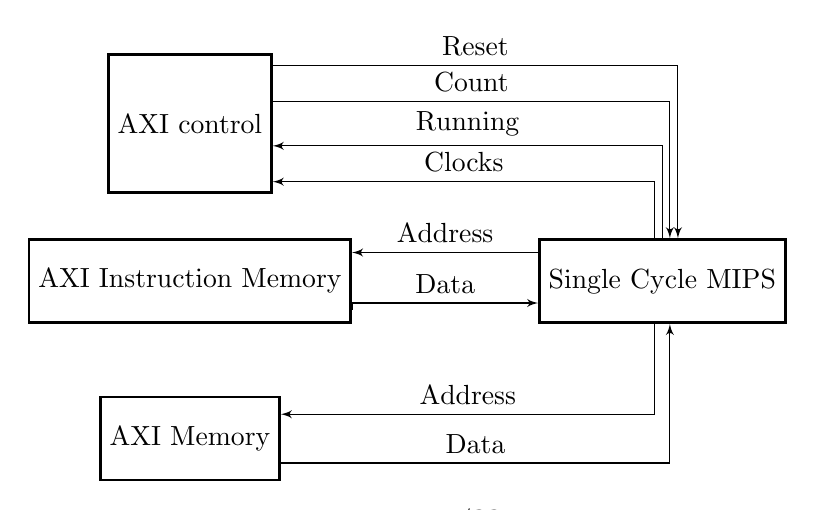
\begin{tikzpicture}
        \node[block, minimum height=5em] (control) at (0,4) {AXI control};
        \node[block] (instruction) at (0,2) {AXI Instruction Memory};
        \node[block] (memory) at (0,0) {AXI Memory};
        \node[block] (mips) at (6,2) {Single Cycle MIPS};

        \path[draw, ->] (control.35) -| node[near start, above]{Reset} (mips.70);
        \path[draw, ->] (control.15) -| node[near start, above]{Count} (mips.80);
        \path[draw, ->] (mips.90) |- node[near end, above]{Running}(control.345);
        \path[draw, ->] (mips.100) |- node[near end, above]{Clocks}(control.325);

        \path[draw, ->] (mips.170) |- node[near end, above]{Address} (instruction.10);
        \path[draw, ->] (instruction.350) |- node[near end, above]{Data} (mips.190);

        \path[draw, ->] (mips.260) |- node[near end, above]{Address}(memory.15);
        \path[draw, ->] (memory.345) -| node[near start, above]{Data}(mips.280);
    \end{tikzpicture}
    \caption{Simplistic overview of how the single cycle MIPS processor should
    be connected to the AXI registers.}
    \label{fig:single-cycle-axi}
\end{figure}

Once the AXI IP have been generated, I integrate it into a block design.  The
procedure is the same, as with the Logic Gates. I do need to add an additional
IP: the clocking wizard. This IP takes an input clock signal and either
multiplies it, or divides it. In this case, I need to divide it. The ZedBoard
has a 100 mhz clock signal, which the FPGA can use. However, as stated before,
I know that the single cycle MIPS processor could be clocked at 5 mhz. As such,
the clocking wizard takes the 100 mhz signal and produce a 5 mhz signal.

Once that is in place, I synthesize, place, route and generate bitstream. The
Single Cycle processor with the AXI interface uses 22\% of the logic available
on the ZedBoard. The Single Cycle processor has an approximate power consumption
of 0.147 watts (excluding the ARM processor). The comparison to the reported
values of the other implementations can be seen in Table~\ref{tab:impl-comp}.

Writing the driver for the processor is straightforward:
\begin{enumerate}
    \item Set the control reset register to 1. I.e. resetting the processor.

    \item Load the instructions into the instruction memory registers.

    \item Set the control instruction count register to the amount of instructions.

    \item Set the control reset register to 0. I.e. starting the processor.

    \item Check that the control running register is set to 1.

    \item Wait for the control running register to become 0.

    \item Now the processor have run. The amount of clock ticks it took is in
        the control clocks register, and the result should be in memory
        (depending on the program of course).
\end{enumerate}
The performance of the VHDL implementation on actual hardware, compared to the
SME simulation of the single cycle processor, can be seen in
Table~\ref{tab:single-cycle-hardware}.

\begin{table}
    \centering
    \begin{tabular}{rllllllllllllllll}
        & FPGA &           & SME \\
        \hline
        & \#CT & time (ms) & \#CT & time(ms) & speedup \\
        \hline
        $n$ = 5 & 718 & $\sim$0.1436 & 719 & 516 & 3593.14 \\
        $n$ = 10 & 22572 & $\sim$4.5144 & 22574 & 13012 & 2882.22 \\
        $n$ = 20 & 23068776 & $\sim$4613.7552 & NA & NA & NA \\
        \hline
    \end{tabular}
    \caption{Performance of the Towers of hanoi program with different $n$
    values. CT is clock ticks. The SME benchmark was performed on a laptop
    with an Intel Core i5-5300U (2.3 GHz). The FPGA benchmark was performed on
    a Zynq-7000 All Programmable SoC XC7Z020-CLG484-1. The MIPS processor
    implemented on the FPGA was clocked to 5 MHz. Towers of hanoi was chosen
    due to it being easy to scale up.}
    \label{tab:single-cycle-hardware}
\end{table}

\subsection{Pipelined MIPS processor}
Many of the same steps as with the Single Cycle processor are required for
implementing the Pipelined processor on an FPGA. However, there are a few
differences:
\begin{itemize}
    \item The Register File should have the same read/write order as in
        the original SME implementation. I.e. it should write first, then read.
        Furthermore, it should now perform all of its actions, on the falling
        edge of the clock.

    \item Within the \texttt{switch} statement of the ALU, all the cases which
        write to the HILO register, should only write on the falling edge of
        the clock.

    \item The Memory should perform all its computations on the falling edge of
        the clock.
\end{itemize}
Other than these differences, the Pipelined processor can be implemented on the
FPGA, in the same manner as with the Single Cycle processor. I was able to clock
it at 68.9776 MHz. As such, pipelining the processor yielded a $\sim$1379\%
speedup. The placed and routed Pipelined processor uses 24\% of the logic
available on the ZedBoard. The Pipelined processor has an approximate power
consumption of 0.019 watts. The comparison to the reported values of the other
implementations can be seen in Table~\ref{tab:impl-comp}.

\subsubsection*{Implementing Block RAM}
Another advantage gained by pipelining the processor, is the option to use block
RAM as memory instead of registers. In the Single Cycle processor,
the instruction had to be read, computed and possibly go through memory in the
same clock cycle. However, block RAM has a delay of one clock cycle, before the
data is ready. As such, it could not be used in the Single Cycle processor.
However, in the Pipelined processor, both the data from the Instruction Memory
and Memory, are not needed until the following clock cycle. As such, I can use
block RAM to get more memory.

I start by adding two new SME processes: InstructionBRAM and MemoryBRAM. Both
of these are \texttt{SimulationProcess}es. As such, they are both clocked
processes and they will not be transpiled. Then I add new busses, which go from
the old processes, to the new processes. The logic in the old processes
just forwards the their input to these new busses. The logic in the new
processes is the same as the previous logic in the old processes. Finally, the
output which previously entered the following pipe, should now go straight to
the receipients. This is due to the delay in the Block Memory, which gives the
same delay as the pipes did.

Once the SME simulation has run and transpiled, the VHDL is entered in a new
project in Vivado. Within this project, I create a new block design. This block
design consists of four modules: the Pipelined processor, two Block Memory
generators and a constant. The two Block Memory modules are connected to the
processor, and the constant is connected to the two Block Memory modules, in
order to keeping the ports used by the processor always enabled. The processor
and the Block Memory generators share the same clock and reset signal.

For easy testing the block design, the Instruction Memory can be initialized
with the use of a \texttt{coe} file. The format of the \texttt{coe} file is
very simple: first there is a line specifying the radix (base) of the numbers,
followed by an array describing the data. E.g. some of the \texttt{coe} file
for the fibonacci program would be
\begin{lstlisting}
memory_initialization_radix=16;
memory_initialization_vector=
34080001,
34090001,
...
00000000;
\end{lstlisting}
I chose to still have dedicated instruction and data memory, as I then did not
have to change any of the compiled programs and due to it resembling the L1
cache of a modern processor. Furthermore, this design makes it easier to extend
with an AXD interface, as Vivado has a Block Memory AXI Controller IP. Each of
the Block Memory Modules can have a maximum of two ports. As such, if I had
gone with the single Block Memory approach, the two ports would already be in
use by the processor.

Once the block design have been constructed, it is time to synthesize, place
and route the design. However, there is a problem when doing this. In the first
version I made, the VHDL had the \texttt{EX\_Pipe\_JALOut} bus, which both goes
to internal processes and outside the network as an top-level bus. Vivado did
not like this particular setup. To solve it, I made an internal signal in VHDL,
to which the processes write and read from. Futhermore, the signal also goes to
the top-level output bus. This does not change the structure of the network,
but satisfies Vivado.

Once the block design could be synthesized, placed and routed, I was able to
clock the processor at 71.429 MHz. The increased clock is due to the Block
Memory. The Block Memory is rated to handle severel hundreds MHz~\cite{ref:bram}
and are as such not even close to being a bottleneck in my design. When the
Instruction Memory and Memory consisted of registers, the path through the
registers was longer, than the path to the Block Memory. Furthermore, since
both have been moved to Block Memory, the logic used by the project have
decreased to use 6\% of the available logic on the ZedBoard. However, the
processor now uses 7\% of the available Block Memory on the Zedboard, making it
the new bottleneck for having multiple cores. The Pipelined processor using
Block Memory has an approximate power consumption of 0.041 watts. The
comparison to the reported values of the other implementations can be seen in
Table~\ref{tab:impl-comp}.

\begin{table}
    \centering
    \begin{tabular}{lllll}
        \hline
        Design           & Clockrate & Memory & Utilization & Power \\
        \hline
        Logic Gates      & N/A & N/A  & 4 & 0.001 \\
        Logic Gates AXI  & 100 & 0.02 & 1 & 0.006 \\
        Single Cycle     & 5   & 0.19 & 14 & 0.001 \\
        Single Cycle AXI & 5   & 1    & 22 & 0.147 \\
        Pipelined        & 68.98 & 0.19 & 24 & 0.019 \\
        Pipelined BRAM   & 71.43 & 64   & 7  & 0.041 \\
        \hline
    \end{tabular}
    \caption{Comparison table of the reported values of the different
        implemented designs. All of them have been made with the ZedBoard as
        the target board. Clockrate is in megahertz. Memory is in kilobytes.
        Utilization is the maximum utilization metric in percent. Power is in
        watts.}
    \label{tab:impl-comp}
\end{table}


\newpage
\section{Conclusion}
I have succesfully implemented a MIPS processor in the SME programming model,
in the timeframe of $\sim$2 months. This shows that the SME model is
suitable for designing hardware, with the prior knowledge of the CSP model,
hardware organization and software development.

Furthermore, by extending the accepted instruction set, and by pipelining the
processor, I have shown that extending the initial design in order to gain
increased performance or additional functionality, is possible.

I have also shown that SME indeed can be transpiled into functioning VHDL, with
a small amount of extra work. The extra actions are however simple enough, such
that they could be implemented in a future version of SME.

As such, with the material in this thesis, a computer science student, such as
myself, should be able to construct specialized hardware by using SME, in the
timeframe of a university course.

%As such, with the material in this paper, everyone with a computer science
%background should be able to construct specialized hardware by using SME.


%\newpage
\section{Future work}
The initial step would be to add an AXI interface to the Pipelined processor.
The approach is the same as with the single cycle processor. It would be
interesting to see whether or not the increased clock is applicable to the
additional AXI interface.
% The initial step would be to synthesize and implement the pipelined processor.
% Given that I have already stated the approach for the single cycle processor,
% this should not be too hard. It could be interesting to see, if it can be
% clocked higher and in that case how much. Furthermore, it would also be more
% usable, as it should have access to more memory.

Inspired by the manycore architecture of the SW26010 processors in the
TaihuLight supercomputer~\cite{ref:supercomputer}, I want to see how many
cores I am able to fit onto a single FPGA. By doing this, I also want to
introduce scratchpad memory, instead of focusing on the traditional memory
hierarchy, as this is what is being used in the SW26010.

It would also be interesting to extend the processor core, to a superscalar
processor, i.e. by introducing multiple execution paths. This could both be by
introducing additional ALUs, e.g. floating point, or by introducing
coprocessors, which are specialized for certain tasks, such as the SME network
of a student project, which solved partial differential equations and fast
fourier transforms.

A final suggestion would be to extend the processor with the required
components, such that a minimal operating system could be compiled and run on
the processor. This would be useful in specialized hardware, if a device should
run purely in its own environment.


\newpage
%\section{References}
%\begin{thebibliography}{9}
    \bibitem{ref:sme} Brian Vinter \& Kenneth Skovhede. \it{Synchronous Message
        Exchange for Hardware Designs}. \copyright\ The authors and Open
        Channel Publishing Ltd. 2014.
    \bibitem{ref:csp} C.A.R. Hoare. \it{Communicating Sequential Processes}.
        \copyright\ ACM 1978
    \bibitem{ref:ark} David A. Patterson \& John L. Hennessy. \it{Computer
        Organization and Design - The Hardware/Software Interface (Revised 4th
        edition)}.  \copyright\ Elsevier 2012
    \bibitem{ref:diku} Maskinarkitektur (ARK) 2013/2014
        \url{http://kurser.ku.dk/course/ndaa04009u/2013-2014}
    \bibitem{ref:logic} Introduction to Combinational Logic Functions
        \url{https://www.allaboutcircuits.com/textbook/digital/chpt-9/combinational-logic-functions/}
\end{thebibliography}


\bibliographystyle{unsrt}
{\small\bibliography{biblio}}

\appendix
\section{Guide til strukturen på github!}

\end{document}
